\setcounter{chapter}{8}
\chapter{Metrische Räume}
Wir haben schon des Öfteren den Begriff des ''Abstands'' verwendet, wobei wir uns direkt die Betragsfunktion oder den Pythagoras zunutze gemacht haben. Dies ist jedoch eine von vielen Weisen, einen Abstand mathematisch zu formulieren. 

Wie genau dieser Abstand bestimmt werden kann, hängt von den zugrundeliegenden mathematischen Strukturen ab. Je nach dem, wie viel gegeben ist, können wir eine der folgenden Strukturen betrachten: Die \textbf{Norm}, die \textbf{Metrik} und die \textbf{Topologie}, die eine abstrakter als die vorherige:

\begin{itemize}
    \item Bei \textbf{Normen} halten wir uns in den uns bekannten Vektorräumen auf, in welcher wir die Länge der Vektoren bestimmen können.
    \item Wollen wir nun unabhängig von Vektorräumen Abstände zwischen Elementen definieren, so können wir dies auf der nächsten Abstraktionsebene der \textbf{Metriken} mit einer Abstandsfunktion oder eben \textbf{Metrik} machen.
    \item Das ist Mathematikern aber zu wenig abstrakt, denn was ist, wenn wir keine Ordnung haben, mit der wir die Distanz ausdrücken und vergleichen können? Man kann also zu guter Letzt die Distanz rein mengentheoretisch als \textbf{Topologie} von einer Menge $X$ definieren. Dabei ist die Topologie eine Menge, die \textit{offene} Teilmengen von $X$ besitzt. Sehr hand-wavy ausgedrückt werden Elemente der ''ähnlichen Distanz'' zu Elementen der Topologie gruppiert.
\end{itemize}

Man könnte erkannt haben, dass eine Norm gewissermassen auch eine Metrik und Topologie ist resp. eine Metrik auch eine Topologie ist -- es gibt also eine Hierarchie zwischen den Begriffen:

$$\text{Norm} \xrightarrow{\text{induziert}}\text{Metrik} \xrightarrow{\text{induziert}}\text{Topologie}$$

Falls also eine Eigenschaft für eine zugrundeliegende Struktur gilt, i.e. Metrik, dann gilt es auch für die darüberliegenden, i.e. Norm. 

\section{Norm}
Beginnen wir also mit den uns bereits bekannten Vektorräumen. Wenn wir mit vektoriellen Werten rechnen wollen wir je nach dem eine Funktion haben, die die Länge der Vektoren bestimmen kann. Solche Funktionen nennen wir \textbf{Normen} und sie sollen folgende Eigenschaften besitzen:

\begin{definition}{Norm}{}
Sei $V$ ein Vektorraum über den Körper $K = \R$ oder $\C$. Eine \textbf{Norm} (Länge) auf $V$ ist eine Abbildung
\begin{align*}
    \Nrm: V &\to \R_{\geq 0}\\
    v &\mapsto \norm{v}
\end{align*}
sodass gilt:
\begin{enumerate}[label=N\arabic*)]
    \item $\norm{\lambda x} = \abs{\lambda} \cdot \norm{x}$ für alle $\lambda \in K, x \in V$ \hfill \textit{(Homogenität)}
    \item $\norm{x} = 0 \iff x = 0$ \hfill \textit{(Definitheit)}
    \item $\forall x,y \in K: \norm{x+y} \leq \norm{x} + \norm{y}$ \hfill \textit{(Dreiecksungleichung)}
\end{enumerate}
Einen Vektorraum mit einer Norm $(V, \Nrm)$ nennen wir einen \textbf{normierten Vektorraum}.
\end{definition}

\begin{example} \label{ex_norm_vr}Hier nun einige Beispiele von verschiedenen Normen auf Vektorräumen:
\begin{enumerate}[label=(\alph*)]
    \item Euklidische Norm auf $\R^n, \C^n$: $\norm{x}_2 = \sqrt{\abs{x_1}^2+...+\abs{x_n}^2}$
    \item Maximumsnorm: $\norm{x}_\infty = \max\{\abs{x_1},...,\abs{x_n}\}$
    auf $\R^n, \C^n$. Axiome folgen aus den Axiomen für die Betragsfunktion.
    \item Eins-Norm: $\norm{x}_1 = \sum_{i=1}^n \abs{x_i}$ 
\end{enumerate}
\end{example}

Im Beispiel haben wir bereits die Notation $\Nrm_p$ für Normen verwendet. Das $p \in \N$ spezifiziert dabei, zu welcher Potenz die Norm berechnet wird:
\begin{definition}{$p$-Norm}{}
 Sei $x \in K^n$, dann gilt:
$$\norm{x}_p = \sqrt[p]{x_1^p+x_2^p+...+x_n^p}$$
Für unendlich-dimensionale Vektoren, z.B. Funktionen $f: [a,b] \to \R$ oder $\C$ gilt:
$$\norm{f}_p = \sqrt[p]{\int_a^b\abs{f(x)}^p dx}$$
Der Fall $p=\infty$ entspricht dabei dem Supremum des Koordinateneinträge resp. der Funktion.
\end{definition}
Somit bezeichnet also $p=2$ die uns bekannte euklidische Norm.

Wir können aber auch unendlich-dimensionale Vektorräume betrachten, zum Beispiel \textbf{Funktionenräume}:
\subsection{Funktionenräume}
Wir wollen also die Menge $C([a, b]) = \{\text{Menge aller stetigen Funktionen } f : [a,b] \to \R \text{(oder $\C$)}\}$  mit einem Begriff für Distanz versehen. Dabei können wir, wie wir bei den endlichen Vektorraum-Normen bereits gesehen haben, die Norm unterschiedlich definieren. Wir wollen zwei gängige Varianten für Funktionenenräume einführen:

\begin{definition}{Supremum-Norm}{}
Für $f \in C([a,b])$ und $x \in [a.b]$ ist die $\sup$-Norm definiert als:
\begin{align*}
    \norm{f}_\infty &= \sup\{\abs{f(x)}, x \in [a,b]\} =: \sup\abs{f(x)}\\
    &= \max\abs{f(x)} \geq 0
\end{align*}
Wobei die zweite Gleichheit aus der Eigenschaft von stetigen Funktionen auf kompakten Intervallen folgt.
\end{definition}
Wir können zeigen, dass $\norm{f}_\infty$ auch tatsächlich eine Norm ist:
\begin{enumerate}[label=N\arabic*)]
    \item $\lambda \in \R : \norm{\lambda f}_\infty = \abs{\lambda} \cdot \norm{f}_\infty$ 
    \item $\norm{f} = 0 \iff \max \abs{f(x)} = 0 \iff f=0$
    \item $\norm{f + g}_\infty = \max \abs{f(x) + g(x)} \leq \max\left(\abs{f(x) + g(x)}\right) \leq \max \abs{f(x)} + \max \abs{g(x)}  = \norm{f}_\infty + \norm{g}_\infty$
\end{enumerate}

\subsubsection{Gleichmässige Konvergenz}\label{cha_funktionenraum_glm_konvergenz}
Mit einer Norm können wir auch eine Konvergenz von Funktionen definieren. Was wir also ganz mühsam im Kapitel \ref{cha_funktionenfolgen} definiert haben, ist hier dasselbe Konzept wie das berechnen der Länge von Vektoren:

Sei $(f_n)$ eine Folge im Funktionenraum $C([a,b])$.
$$ f_n \to f \quad (n \to \infty)$$
bedeutet dann
\begin{align*}
    \norm{f_n - f}_\infty &\longrightarrow 0 \quad (n \to \infty)\\
    \max \abs{f_n(x) -f(x)} &\longrightarrow 0 \quad (n \to \infty)
\end{align*}
In der uns vertrauten $\varepsilon$-Terminologie kann man das auch wie folgt ausdrücken:
$$\forall \varepsilon >0\ \exists n_0 \in \N : \forall n\geq n_0, \forall x \in [a,b]: \abs{f_n(x) - f(x)} < \varepsilon$$
Wir sehen also, dass $f_n$ gegen $f$ bezüglich der Norm $\Nrm_\infty$ genau dann konvergiert, wenn $f_n$ gleichmässig gegen $f$ konvergiert. Somit ist es also eine alternative, kompaktere Definition der gleichmässigen Folgenstetigkeit.

Eine andere Norm für Funktionenräume bildet die folgende:
\begin{definition}{Eins-Norm}{}
Für $f \in C([a,b])$ und $x \in [a,b]$ ist die Eins-Norm definiert als:
$$\norm{f}_1 = \int_a^b \abs{f(x)} dx$$
\end{definition}
Es wir also der Betrag der Fläche unter der Funktion auf $[a, b]$ als Norm verwendet. Auch hier können wir zeigen, dass es sich um eine Norm handelt:

\begin{enumerate}[label=N\arabic*)]
    \item $\norm{\lambda f}_1 = \int_a^b \abs{\lambda f(x)}dx = \int_a^b \abs{\lambda} \cdot \abs{f(x)}dx = \abs{\lambda} \cdot \norm{f}_1$ 
    \item $\norm{f}_1 = \int_a^b \abs{f(x)}dx = 0 \iff f=0$
    \item $\norm{f + g}_1 = \int_a^b \abs{f(x) + g(x)}dx \leq \int_a^b \left(\abs{f(x)} + \abs{g(x)}\right) dx = \int_a^b\abs{f(x)}dx + \int_a^b \abs{g(x)}dx = \norm{f}_1 + \norm{g}_1$
\end{enumerate}

\subsubsection{Konvergenz im Mittel}
Die Konvergenz, die durch die Eins-Norm definiert wird, nennen wir die \textbf{Konvergenz im Mittel}:
\begin{definition}{Konvergenz im Mittel}{}
Sei $(f_n)$ eine Folge im Funktionenraum $C([a,b])$. Bei der Konvergenz im Mittel gilt:
$$f_n \to f  \quad (n \to \infty)\iff \int_a^b\abs{f_n - f(x)} dx \to 0 \quad (n \to \infty)$$
\end{definition}
Diese Konvergenz ist weniger einschränkend als die gleichmässige Konvergenz von der $\sup$-Norm und folgt auch aus dieser:
$$\text{gleichmässige Konvergenz} \implies \text{Konvergenz im Mittel}$$
da mit $\norm{f_n - f}_\infty < \frac{ \varepsilon}{b-a}$ von der gleichmässigen Konvergenz folgende Aussage gilt:
$$\varepsilon > (b-a) \norm{f_n - f}_\infty \geq \int_a^b \abs{f_n(x) -f(x)}dx = \norm{f_n-f}_1$$
$\norm{f_n - f}$ bezeichnet per Definition dieser Norm die grösste Differenz zwischen $f_n$ und $f$, somit ist die Differenz des Integrals auf dem gesamten Intervall höchstens $(b-a)$-mal so gross wie die grösste Differenz $\norm{f_n - f}$; daher die entsprechene Wahl des $\varepsilon$.

Auch hier sehen wir, dass $f_n$ gegen $f$ bezüglich der Norm $\Nrm_1$ genau dann konvergiert, wenn $f_n$ punktweise gegen $f$ konvergiert. Somit ist es also eine alternative, kompaktere Definition der punktweisen Folgenstetigkeit.

Das Beispiel \ref{ex_grenzfunktion} konvergiert daher im Mittel, jedoch wie bereits gezeigt, nicht gleichmässig. Intuitiv lässt sich das daran erkennen, dass die Fläche unter der Funktion beliebig klein gemacht werden kann.

\subsection{Äquivalenz von Normen}\label{cha_eq_norms}
Wir haben gesehen, dass wir verschiedene Normen definieren können, die an der Oberfläche in unterschiedlichen Konvergenzverhalten äussert. Wir können aber zeigen, dass von einigen Normen die zugrundeliegende Mechanismus der Konvergenz derselbe ist. Wir wollen daher die folgende Äquivalenz zwischen Normen definieren:
\begin{definition}{}{}
Zwei Normen $\Nrm, \Nrm'$ auf $V$ heissen \textbf{äquivalent} $\Nrm \sim \Nrm'$, falls es Zahlen $c_1, c_2 > 0$ gibt, so dass
$$c_1 \norm{x}' \leq \norm{x} \leq c_2 \norm{x}'$$
für alle $x \in V$ gilt.
\end{definition}
Wir können zeigen, dass es sich bei $\sim$ auch um eine Äquivalenzrelation handelt:
\begin{exercise}[Äquivalenzrelation] $\sim$ ist eine Äquivalenzrelation auf der Menge der Normen auf $V$. \todo{Beweis einfügen}
\end{exercise}

\begin{example} Hier einige bereits bekannte Normen im Vektorraum $\R^n$, welche äquivalent zueinander sind:
\begin{itemize}
    \item $\Nrm_2 \sim \Nrm_\infty$ (Es gilt mit $x_i = \max \{x_1, ..., x_n\} = \norm{x}_\infty $: $\norm{x}_\infty \leq \sqrt{x_1^2 +...+x_n^2} \leq \sqrt{n} \norm{x}_\infty$)
    \item $\Nrm_1 \sim \Nrm_\infty$ (Es gilt: $\norm{x}_\infty \leq \abs{x_1}+...+\abs{x_n} \leq n \norm{x}_\infty$)
\end{itemize}

\end{example}

Follow-up: Wir werden im  Abschnitt \ref{cha_eq_norms_topology} zeigen, dass eine solche Äquivalenz auf dieselbe Topologie zurückzuführen ist.

\section{Metrik}
Nun wollen wir den ersten Schritt der Abstraktion wagen und uns vom Konzept der Vektorräume entfernen. Wir wollen stattdessen eine allgemeinere Abstandsfunktion einführen, welche die Elemente einer Menge mit folgenden Eigenschaften auf $\R$ (oder einen anderen geordneten Körper) abbildet:
\begin{definition}{Metrik}{}
Sei $X$ eine Menge, dann ist eine \textbf{Metrik} eine Abbildung
$$d: X\times X \to \R_{\geq 0}$$
sodass Folgende Axiome erfüllt sind:
\begin{enumerate}[label=M\arabic*)]
    \item Für alle $x,y \in X : d(x,y) = d(y,x)$ \hfill \textit{(Symmetrie)}
    \item $d(x,y) = 0 \iff x=y$
    \item $\forall x,y,z \in X: d(x,z) \leq d(x,y) + d(y,z)$ \hfill \textit{(Dreiecksungleichung)}
\end{enumerate}
Eine Menge $X$ die mit einer Metrik $d$ versehen ist, nennen wir \textbf{metrischen Raum} und notieren dies als Tupel: $(X, d)$
\end{definition}

Man erkennt sofort nur schon durch Vergleichen der Axiome von Normen und Metriken, dass jede Norm auch eine Metrik ist. Deswegen werden uns einige der folgenden Beispiele auch sehr bekannt vorkommen:

\begin{example}[Euklidische Metrik] Die uns bekannte Metrik ist die \textbf{Euklidische Metrik}. Für die Menge $X = \R^n$ mit ist die Abstandsfunktion $d$ definiert als:
$$d_E(x,y) = \sqrt{(x_1-y_1)^2+...(x_n-y_n)^2}$$
wobei $x = (x_1, x_2, ..., x_n) \in \R^n$ und $y = (y_1, y_2, ..., y_n) \in \R^n$ gilt.
\end{example}

\begin{example}[Manhattan-Metrik] Befindet man sich in einer Stadt mit schachbrettartig angeordneten Blöcken, i.e. Manhattan, kann man sich nur in orthogonal zueinander liegende Richtungen bewegen. Man enthält also folgende Metrik für die zurückgelegte Distanz (mit $X = \R^n$ und $x,y \in X$):
$$d_M(x,y) = \abs{x_1 - y_1} + ... + \abs{x_n - y_n}$$
M1 und M2 kann man selber schnell verifizieren, wir zeigen M3:
$$d_M(x,z) = \sum_{i=1}^n \abs{x_i-z_i} \leq \sum_{i=1}^n \abs{x_i-y_i} + \abs{y_i-z_i} = d_M(x,y) + d_M(y,z)$$

\end{example}

\begin{example}[Französische Eisenbahnmetrik] Im Frankreich der Industrialisierung gab es vor allem Eisenbahnlinien, welche direkt aus der Agglomeration ins Zentrum Paris führten, i.e. waren radial mit Paris als Zentrum. Wollte man von einer Station zur anderen, musste man in Paris umsteigen --- es sei denn, die Endstation liegt genau auf der selben radialen Bahnlinie, dann ist der Weg kürzer. Wir können diese Metrik daher als Metrik von $X = \C$ mit $z,w \in \C$ definieren:
$$d_{SNCF}(z,w) = \begin{cases} \abs{z-w} &, \text{falls $z,w$ auf derselben Gerade durch 0 liegen} \\ \abs{z} + \abs{w} & , \text{sonst} \end{cases}$$
\end{example}

\begin{example}[Bogenlänge auf Kugel] Sei $X = \set{(x,y,z) \in \R^3}{x^2+y^2+z^2=1}$ die Einheitskugel im $\R^3$. Wir definieren Metrik wie folgt:
$$d_K(a,b) = \text{Länge eines kürzesten Grosskreisbogen zwischen $a$ und $b$}$$
wobei der Grosskreisbogen von $a$ und $b$ die Bogenlänge des Kreises ist, der durch den Schnitt von $X$ und der Ebene durch $a,b$ und 0 ist:
$$d_K(a,b) = \arccos{a\cdot b}$$
\end{example}
\begin{exercise} Verifiziere M1 -- M3 für die $d_{SNCF}$ und für $d_K$.\end{exercise}

\subsection{Teilraum}
Wir haben bis jetzt stets Räume direkt mit einer Metrik definiert, jedoch können wir auch einen metrischen Raum auf einen \textbf{Teilraum} einschränken, wobei die Metrik selber auf diese Teilmenge ''vererbt'' wird:

\begin{definition}{Teilraum}{}
Ein \textbf{Teilraum} oder \textbf{Unterraum}\footnote{Nicht zu verwechseln mit dem Untervektorraum der linearen Algebra.} von einem metrischen Raum $(X,d)$ ist eine Teilmenge $Y \subseteq X$ mit der Metrik
$$d\vert_{Y\times Y}: Y \times Y \to \R_{\geq 0}$$
\end{definition}

\begin{example}[Euklidische Metrik auf Kreis] Sei die Menge $S^1 \subseteq \R^2$, $S^1 = \set{(x,y)}{x^2+y^2=1}$ der Einheitskreis mit der Euklidischen Metrik aus dem $\R^2$. Dann bezeichnet $d(x,y)$ mit $x,y \in S^1$ die Länge der Sehne zwischen $a$ und $b$.
\end{example}

Wir werden hauptsächlich Fälle betrachten, welche Teilräume von den normierten Vektorräumen $\R^n$ oder $\C^n$ mit der euklidischen Norm/Metrik sind. Zwar sind diese Teilmengen selber nicht unbedingt Vektorräume, jedoch kann man die Metrik des Vektorraums darauf verwenden.

\subsection{Induzierte Metrik}

Wie wir bereits angedeutet haben, induziert eine Norm stets eine Metrik. Dies bedeutet also, dass man mit der Norm eines Vektorraums auch eine Metrik auf dem Raum definieren kann:

\begin{satz}{Induzierte Metrik}{}
Sei $(V, \norm{\ \cdot \ })$ ein normierter Vektorraum. Dann definiert
$$d(x,y) = \norm{x - y}$$
mit $x,y \in V$ eine Metrik auf $V$.
\end{satz}
Wir wollen nun verifizieren, dass eine Norm resp. normierte Vektorräume die Axiome der Metrik M1 -- M3 erfüllen: 
\begin{proof} Sei $d: X \times X \to \R_{\geq 0}$

(M1) Es gilt: 
$$d(y,x) = \norm{y-x} = \norm{(-1)(x-y)} \stackrel{N1}{=} \underbrace{\abs{-1}}_{1} \norm{x-y} = d(x,y)$$
(M2) Es gilt:
$$d(x,y) = 0 \iff \norm{x-y}=0 \stackrel{N2}{\iff} x-y = 0 \iff x= y$$
(M3) Es gilt:
$$d(x,z) = \norm{x-z} = \norm{x-y+y-z} \stackrel{N3}{\leq} \norm{x-y} + \norm{y-z} = d(x,y) + d(y,z)$$
\end{proof}

\begin{lemma}{Translationsinvarianz}{}
Sei $\Nrm$ eine Norm vom Vektorraum $V$, dann ist die induzierte Metrik $d_{\Nrm}$ translationsinvariant:
$$\forall a \in V: d_{\Nrm}(x,y)=d_{\Nrm}(x+a,y+a)$$
\end{lemma}
\begin{proof}
$d_{\Nrm}(x,y) = \norm{x-y} = \norm{(x+a)-(y+a)}=d_{\Nrm}(x+a,y+a)$
\end{proof}

\begin{remark}
Wir erkennen, dass die Manhattan-Metrik $d_M$ durch die Eins-Norm induziert wird, siehe Beispiel \ref{ex_norm_vr} c). Hingegen wird die Französische Eisenbahnmetrik durch keine Norm induziert, denn sie erfüllt im Allgemeinen nicht die Translationsinvarianz.
\end{remark}

\subsection{Konvergenz}
Wir haben die Konvergenz bereits in beliebigen Mengen definiert, nun wollen wir aber allgemeiner den Begriff der Konvergenz für beliebige metrische Räume einführen, um z.B. auch Konvergenz in Funktionenräumen oder in höherdimensionalen Vektorräumen betrachten zu können. Dabei werden uns sehr viele Begriffe bekannt vorkommen, da diese schon sehr ähnlich im Rahmen der bereits besprochenen Konvergenz definiert wurde.

\begin{definition}{Konvergenz im metrischen Raum}{}
Sei $(X, d)$ ein metrischer Raum und $(x_n)_n$ eine Folge/Abbildung von $n \in \N \to x_n \in X$. Die Folge $(x_n)_n$ konvergiert gegen $x \in X$, falls es zu jedem $\varepsilon > 0$ ein $n_0 \in \N$ gibt, sodass
$$\forall n \geq n_0: d(x_n,x) < \varepsilon$$
Wir nennen $x$ den \textbf{Grenzwert} und schreiben
$$x = \lim_{n \to \infty} x_n \qquad \text{oder} \qquad x_n \to x \quad (n \to \infty)$$
\end{definition}

\begin{remark}
Dabei gilt $x = \lim_{n \to \infty}x_n$ genau dann, wenn $\lim_{n \to \infty} d(x_n,x) = 0$ gilt.
\end{remark}

Wie bei den uns bereits bekannten Grenzwerten, sind diese Grenzwerte ebenfalls eindeutig:
\begin{lemma}{Eindeutigkeit des Grenzwertes}{}
Der Grenzwert einer Folge ist eindeutig.
\end{lemma}

\begin{proof}
Im Grunde ist das derselbe Beweis wie für Grenzwerte in $\R$ oder $\C$: Seien $x\neq y$ beides Grenzwerte der Folge $(x_n)$, dann gilt für ein $\varepsilon > 0$ und ein $n \in \N$ gross genug sowohl $d(x_n,x) < \frac{\varepsilon}{2}$ als auch $d(x_n,y) < \frac{\varepsilon}{2}$. Dies ist aber ein Widerspruch mit der Dreieckungleichung, wenn wir $\varepsilon = d(x,y) > 0$ wählen:
$$\varepsilon = d(x,y) \leq d(x_n, x) + d(x_n, y) < \frac{\varepsilon}{2} + \frac{\varepsilon}{2} = \varepsilon$$
\end{proof}

Wir werden in folgendem Beispiel sehen, dass die Wahl der Norm einen wesentlichen Einfluss auf den Begriff der Konvergenz hat:

\begin{example}[Normen und Konvergenzen] Wir betrachten die Folge $(e^{i\frac{1}{n}})_n$ in $\C$, die eine Folge auf dem Einheitskreis bezeichnet, die sich der $1$ nähert. Mit der euklidischen Norm $\Nrm_2$ erhalten wir als Grenzwert:
$$\lim_{n \to \infty} e^{i\frac{1}{n}} = 1$$
da $\abs{e^{i\frac{1}{n}} - 1} = \sqrt{(\cos \frac{1}{n} - 1)^2 + \sin^2\frac{1}{n}} \to 0$ gilt. 

Für die Metrik $d_{SNCF}$ jedoch konvergiert diese Folge nicht, da immer $d_{SNCF}(e^{i\frac{1}{n}}, 1) = 2$ gilt.
\end{example}

\section{Topologie von metrischen Räumen}
Nun wollen wir uns der letzten Abstraktionsebene, der \textbf{Topologien}, widmen. Wir werden dabei --- wie der Titel des Abschnittes schon vermuten lässt --- immer wieder auf Konzepte von metrischen Räumen zurückgreifen. Es wäre aber möglich, all diese topologischen Begrifflichkeiten ausschliesslich mengentheoretisch zu definieren. 

Zuerst wollen wir jedoch noch die Grundbegriffe der \textbf{Umgebung} und der \textbf{Offenheit von Mengen} einführen:

\subsection{Umgebungen}
\begin{definition}{Umgebung}{}
Sei $(X,d)$ ein metrischer Raum und $\varepsilon > 0$. Die \textbf{$\varepsilon$-Umgebung} von $x \in X$ ist
$$B_\varepsilon(x) = \set{y \in X}{d(x,y)<\varepsilon}$$
Wir haben diese Umgebung auch als \textbf{offenen Ball} von Radius $\varepsilon$ um $x$ bezeichnet. 

Die \textbf{Umgebung} [neighbourhood] von $x \in X$ ist eine Teilmenge von $X$, die für ein $\varepsilon > 0$ eine $\varepsilon$-Umgebung enthält. 
\end{definition}
Dabei kommt es bei Umgebungen nicht darauf an, ob der Rand in der Menge ist oder nicht.

\begin{example} Einige Beispiele zu Umgebungen verschiedener Metriken:
\begin{itemize}
    \item $X=\R, B_\varepsilon(x) = (x-\varepsilon, x+\varepsilon)$
    \item $X=\R^2$ mit euklidischer Metrik. $B_\varepsilon(x)$ bezeichnet die offene Kreisscheibe mit Radius $\varepsilon$ um $x$
    \item $X=\R^2$ mit Manhattan-Metrik. $$B_\varepsilon(x) = \{y \in \R^2 \text{ mit } \norm{y-x}_1 = \abs{y_1-x_1} + \abs{y_2-x_2} < \varepsilon\}$$ bezeichnet einen offenen Rhombus mit Breite und Höhe $2\varepsilon$ um den Punkt $x$.
    \item $X = \R^2$ mit $\sup$-Metrik. $$B_\varepsilon(x) = \{y \in \R^2\text{ mit }\norm{y-x}_\infty = \max\{\abs{y_1-x_1}, \abs{y_2-x_2} < \varepsilon\}$$ bezeichnet ein Quadrat mit Seitenlänge $2\varepsilon$ um den Punkt $x$.
\end{itemize}
\end{example}

\subsection{Offene Mengen}\label{cha_offenheit}
Nun wollen wir die Begriffe der Offenheit in metrischen Räumen definieren:

\begin{definition}{Offene Teilmenge}{}
Sie $(X, d)$ ein metrischer Raum, dann ist $U \subseteq X$ \textbf{offen}, falls für alle $x \in U$ eine $\varepsilon$-Umgebung $B_\varepsilon(x)$ mit $\varepsilon >0$ existiert, sodass $B_\varepsilon(x) \subseteq U$ gilt.
\end{definition}
Ein einfaches Beispiel wäre die Teilmenge von $\varepsilon$-Umgebungen. Es folgen daraus einige Lemmata:

\begin{lemma}{Folgerungen}{folgerungen_offenheit}
\begin{enumerate}
    \item $\emptyset, X$ sind offen.
    \item endliche Durchschnitte und beliebige Vereinigungen von offenen Mengen sind offen:
    \begin{enumerate}[label=(\alph*)]
        \item Seien $U_1, ... , U_n$ offen in $X$, dann ist der endliche Schnitt $U_1 \cap ... \cap U_n $ offen.
        \item Sei $(U_i)_{i \in I}$ eine Familie von offenen Mengen, dann ist die Vereinigung offen.
        $$\bigcup_{i\in I}U_i = \set{x \in X}{\exists i:x \in U_i}$$ 
    \end{enumerate}
\end{enumerate}
\end{lemma}
\begin{proof}
\begin{enumerate}
    \item $\emptyset$ ist offen, da jede Aussage für die Elemente der leeren Menge gilt. $X$ ist offen, da jede $\varepsilon$-Umgebung (auch auf dem Rand) per Definition eine Teilmenge von $X$ sein muss, somit ist $X$ auch offen.
    \item \begin{enumerate}[label=(\alph*)]
        \item Seien $U_1, ... , U_n$ offen und $x \in U_1 \cap ... \cap U_n $. Da $U_i$ offen ist, existiert ein $B_{\varepsilon_i}(x) \subseteq U_i$ mit $\varepsilon_i > 0$. Wähle $\varepsilon = \min\{\varepsilon_1, ..., \varepsilon_n\} > 0$, dann gilt $B_\varepsilon(x) \subseteq B_{\varepsilon_i} \subseteq U_i$ für alle $0 \leq i \leq n$. Es gilt $B_\varepsilon \subseteq U_1 \cap ... \cap U_n$, also ist der Schnitt offen.
        \item Für ein $x \in \bigcup_{i\in I}U_i$ finden wir ein $i \in I$, sodass $x \in U_i$ gilt. Wir können also ein $\varepsilon >0$ finden, sodass $B_\varepsilon(x) \subseteq U_i \subseteq \bigcup_{i\in I}U_i$ gilt. Also ist die Vereinigung offen.
    \end{enumerate}
\end{enumerate}
\end{proof}

\begin{remark}
Beim Schnitt von offenen Mengen ist im Allgemeinen die endliche Anzahl Mengen von Wichtigkeit. Dies widerspiegelt sich auch im Beweis, da wir das Minimum für das $\varepsilon$ bestimmen müssen. Bei einem unendlichen Schnitt müssen wir je nach dem das Infimum wählen, wodurch der Schnitt nicht mehr offen ist:
\end{remark}

\begin{example}[unendlicher Schnitt] Sei $X = \R$ und $U_n = (-\frac{1}{n}, \frac{1}{n})$, dann ist der Schnitt aller Mengen nicht offen:
$$\bigcap_{n \in \N} U_n = \{0\}$$
\end{example}

\begin{remark} Des Weiteren ist die Offenheit einer Menge im Allgemeinen abhängig von der Wahl der Metrik:
\begin{example}
Die offene Menge $B_1(1)$ von $(\C, d_{SNCF})$ ist das offene Intervall $(0,2)$. Diese Menge ist jedoch nicht offen bezüglich $(\C, d_E)$, da jeder $\varepsilon$-Schritt entlang der imaginären Achse nicht mehr in der Menge liegt.
\end{example}
Wir werden aber im Abschnitt \ref{cha_eq_norms_topology} sehen, dass äquivalente Normen dieselbe Offenheit beschreiben.
\end{remark}

\subsection{Topologie}
Mit der Offenheit von Mengen können wir nun den Begriff der \textbf{Topologie} definieren:

\begin{definition}{Topologie}{}
Die Menge $\mathcal{U}$ aller offenen Teilmengen eines metrischen Raums $(X,d)$ heisst \textbf{Topologie} von $(X,d)$.

$X$ versehen mit einer Topologie heisst \textbf{topologischer Raum}.
\end{definition}
\begin{remark}
Unabhängig von metrischen Räumen definiert heisst eine Menge $\mathcal{U}$ von Teilmengen einer Menge $X$ \textbf{Topologie}, falls sie die Eigenschaften 1. und 2. des Lemmas \ref{lem:folgerungen_offenheit} zur Offenheit von Mengen erfüllt. Auf diese Weise definierte Topologien müssen nicht unbedingt durch eine Metrik induziert sein, so sind die triviale und die \textsc{Zariski}-Topologie Beispiele für Topologien, denen keine Metrik zugrunde liegt.
\end{remark}

\subsection{Äquivalente Normen und Topologien}\label{cha_eq_norms_topology}
Wir haben im Abschnitt \ref{cha_eq_norms} den Begriff der äquivalenten Normen eingeführt. Nun werden wir zeigen, dass äquivalente Normen auf dieselbe zugrundeliegende Topologie zurückzuführen sind resp. dieselbe Topologie induzieren/definieren:
\begin{lemma}{Äquivalente Normen und Topologien}{}
Äquivalente Normen definierten dieselbe Topologie. Seien $\Nrm, \Nrm'$ äquivalente Normen auf einem Vektorraum $V$, dann gilt:

\centering $U$ offen bezüglich $\Nrm \iff U $ offen bezüglich $\Nrm'$
\end{lemma}

\begin{proof} Wir wollen zeigen, dass offene Mengen bezüglich einer Norm $\Nrm$ auch offen bezüglich einer anderen, äquivalenten Norm $\Nrm'$ sind. Hierfür wollen wir folgende Notation für $\varepsilon$-Umgebungen verschiedener Normen um einen Punkt $x \in V$ verwenden:
\begin{align*}
    B_\varepsilon(x) &= \set{y \in V}{\norm{x-y} < \varepsilon}\\
    B'_\varepsilon(x) &= \set{y \in V}{\norm{x-y}' < \varepsilon}
\end{align*}
Des Weiteren gilt aufgrund der Äquivalenz zwischen $\Nrm$ und $\Nrm'$, dass es zwei Konstanten $c_1$ und $c_2$ gibt, mit welchen für alle $v \in V$ gilt:
$$c_1 \norm{v}' \leq \norm{v} \leq c_2 \norm{v}'$$
Sei also $y \in B'_\varepsilon(x)$, dann folgt aus der Äquivalenz: $\norm{x-y} \leq c_2\norm{x-y}' < c_2 \varepsilon$. Wir erhalten die Bedingung $y \in B_{c_2 \varepsilon}(x)$, also folgt: $B'_\varepsilon(x) \subseteq B_{c_2 \varepsilon}(x)$. Analog dazu folgt aus $y \in B_\varepsilon(x)$ und der Äquivalenz $c_1\norm{x-y}' \geq \norm{x-y} < \varepsilon$, also erhalten wir durch Division mit $c_1$ die Bedingung für $y \in B'_{\frac{\varepsilon}{c_1}}$, also $B_\varepsilon \subseteq B'_{\frac{\varepsilon}{c_1}}$

Sei nun $U\subseteq V$ eine offene Menge bezüglich $\Nrm$, dann gilt für ein $x \in U$:
$$\exists B_\varepsilon(x) \subseteq U \implies B'_{\frac{\varepsilon}{c_2}} \subseteq B_\varepsilon(x) \subseteq U$$
Da aber $x$ ein beliebiges Element aus U ist, ist U auch offen bezüglich $\Nrm'$. Analog dazu ist eine offene Menge $U'\subseteq V$ bezüglich $\Nrm'$ offen bezüglich $\Nrm$. Also definieren äquivalente Normen dieselbe Topologie.
\end{proof}

\subsection{Konvergenz auf Topologien}
Auch auf der Stufe der Topologie können wir wieder den Begriff der Konvergenz definieren --- und das komplett unabhängig von der Metrik oder der Norm. Wir wollen also folgenden Satz zeigen:

\begin{satz}{Konvergenz auf Topologien}{}
Eine Folge $(x_n)_n$ in einem metrischen Raum $(X, d)$ konvergiert gegen $x \in X$ genau dann, wenn für alle offenen Teilmengen $U$, die $x$ enthalten, ein $n_0 \in \N$ existiert, sodass alle Folgeglieder $x_n$ mit $n\geq n_0$ in $U$ liegen:
$$\lim_{n \to \infty} x_n = x \iff \forall U \ni x, U \text{ offen}: \exists n_0 \in \N: \forall n \geq n_0 : x_n \in U$$
\end{satz}
\begin{proof}
($\Longrightarrow$) Die Folge $(x_n)$ konvergiert gegen $x$, also gibt es für jedes $\varepsilon >0$ ein $n_0$, sodass für alle Folgeglieder $x_n$ mit $n \geq n_0$ gilt: $d(x_n, x) < \varepsilon$ oder mit der Umgebung formuliert: $x_n \in B_\varepsilon(x)$. Sei nun die Teilmenge $U$, welche $x$ enthält, offen. Somit finden wir auch eine $\varepsilon$-Umgebung $B_\varepsilon(x)$, sodass für alle $n\geq n_0$ gilt: $x_n \in B_\varepsilon(x) \subseteq U$.

($\Longleftarrow$) Wähle für ein $\varepsilon > 0$ die Umgebung $U = B_\varepsilon(x)$.
\end{proof}

\subsection{Abgeschlossene Mengen}
Mit der Offenheit einer Menge können wir auch die \textbf{Abgeschlossenheit} definieren:
\begin{definition}{Abgeschlossenheit}{}
Die Teilmenge $A \subseteq X$ eines metrischen Raumes $(X,d)$ ist abgeschlossen, wenn das Komplement $X\setminus A = A^C$ offen ist.
\end{definition}
\begin{example}Einige Beispiele mit der euklidischen Metrik im $\R^2$:
\begin{itemize}
    \item $(0,1) \times (0,1)$ ist offen und nicht abgeschlossen.
    \item $(0,1) \times (0,1]$ ist weder offen noch abgeschlossen.
    \item $[0,1] \times [0,1]$ ist nicht offen aber abgeschlossen.
\end{itemize}
\begin{remark}
Es ist zu beachten, dass dies eine ausschliesslich durch die Offenheit des Komplements bestimmte Eigenschaft ist. Es gibt keine Implikation \textit{''$A$ offen $\implies A$ nicht abgeschlossen''} oder dergleichen. Von der Offenheit der Menge selber kann man also nicht auf deren Abgeschlossenheit schliessen und umgekehrt.
\end{remark}
\end{example}

Mit dem Begriff der Konvergenz können wir für die Abgeschlossenheit folgenden Satz formulieren:
\begin{satz}{Grenzwert in abgeschlossenen Mengen}{grenzwert_abgeschlossenen_mengen}
Eine Teilmenge $A \subseteq X$ ist genau dann abgeschlossen, wenn für alle konvergenten Folgen $(x_n)_n$ deren Folgenglieder $x_n$ alle in $A$ liegen, auch der Grenzwert in $A$ liegt:
$$A \text{ abgeschlossen} \iff \forall (x_n)_n \land \set{x_n}{n\in \N} \subseteq A: \lim_{n \to \infty} x_n \in A $$
\end{satz}
Kurz für die Intuition: Wir wissen bereits, dass Folgen in einem offen Intervall, z.B. $x_n = \frac{1}{n} \in (0,2)$, zu einem Grenzwert ausserhalb des Intervalls konvergieren können, im Fall vom Beispiel $\lim_{n \to \infty}x_n = 0 \notin (0,2)$. Wenn das Intervall aber abgeschlossen ist, ist der Rand bereits dabei und man kann eine Grenzwerte ausserhalb davon erreichen. Hier der formale Beweis:
\begin{proof}
Sei $A$ abgeschlossen resp. das Komplement $A^C$ offen und $(x_n)_n$ eine konvergente Folge mit $x_n \in A$ für alle $n$ mit Grenzwert $\lim_{n \to \infty}x_n = x$.

($\Longrightarrow$) Wir nehmen an, dass $x \in A^C$ und führen es zu einem Widerspruch: Da $x \in A^C$ ist und $A^C$ offen ist, kann man ein $n$ finden, sodass $x_n \in A^C$ liegt, also ein Widerspruch zur Annahme.

($\Longleftarrow$) Wir nehmen an, dass $A^C$ nicht offen ist. Somit gibt es ein $x \in A^C$ (auf dem Rand), sodass der Schnitt $A \cap B_{\frac{1}{n}}(x)$ für alle $n \in \N$ nicht-leer ist (d.h. nicht, dass $A^C$ abgeschlossen ist! Falls unklar, siehe Definition von offenen Mengen \ref{cha_offenheit}). Wir konstruieren nun die Reihe mit $x_n \in A \cap B_{\frac{1}{n}}(x)$, somit sind alle Folgenglieder $x_n \in A$, jedoch ist der Grenzwert per Konstruktion $x \in A^C$, also ein Widerspruch.
\end{proof}

\subsection{Innere Punkte, Randpunkte und Abschluss}
Wir wollen nun die Punkte einer Menge anhand ihrer Umgebung charakterisieren:

\begin{definition}{Innerer Punkt, Inneres und Abschluss}{}
Sei $Y \subseteq X$ eine Teilmenge des metrischen Raums $X$. Dann heisst $y \in Y$ \textbf{innerer Punkt} von $Y$, falls $y$ eine komplett in $Y$ enthaltene Umgebung besitzt:
$$Y \text{ abgeschlossen} \iff \forall y \in Y: \exists\varepsilon>0: B_\varepsilon(y) \subseteq Y$$
Das \textbf{Innere} [interior] von $Y$ bezeichnen wir als die Menge aller inneren Punkte von $Y$ und schreiben
$$\mathring{Y} = \{\text{innere Punkte von Y}\}$$
Den \textbf{Abschluss} [closure] von $Y$ bezeichnen wir als die Menge aller Grenzwerte von Folgen in $Y$
$$\quer{Y} = \{\text{Grenzwerte von Folgen in }Y\}$$
\end{definition}
\begin{lemma}{Folgerungen}{}
Wir können zeigen, dass folgende Behauptungen gelten:
\begin{enumerate}[label=\alph*)]
    \item $\mathring{Y}$ ist offen
    \item $\quer{Y}$ ist abgeschlossen
    \item Für alle offenen Mengen $A \subseteq X$ gilt: $A \subseteq Y \iff A \subseteq \mathring{Y}$
    \item Für alle abgeschlossenen Mengen $A \subseteq X$ gilt: $A \supseteq Y \iff A \supseteq \quer{Y}$
\end{enumerate}
\end{lemma}
\begin{proof}
\begin{enumerate}[label=\alph*)]
    \item Folgt direkt aus der Definition von inneren Punkten.
    \item Sei $(x_n)_n$ eine konvergente Folge in $\quer{Y}$, also gilt für alle Folgenglieder $x_n \in \quer{Y}$. Wir wollen zeigen, dass der Grenzwert $\lim_{n \to \infty}x_n = x$ in $\quer{Y}$ liegt. Wir können aufgrund der Konstruktion des Abschlusses $\quer{Y}$ für jedes $n$ ein $y_n \in Y$ finden, sodass $d(x_n, y_n) < \frac{1}{n}$ gilt. Die Folge $(y_n)_n$ liegt in $Y$ und konvergiert ebenfalls gegen $x$:
    $$d(x,y_n) \stackrel{DU}{\leq} \underbrace{d(x,x_n)}_{\to 0} + \underbrace{d(x_n + y_n)}_{<\frac{1}{n} \to 0}$$
    Da $(y_n)_n$ nach $x$ konvergiert, giltju per Definition des Abschlusses $x \in \quer{Y}$.\footnote{Beachte, dass wir Satz \ref{satz:grenzwert_abgeschlossenen_mengen} für diese Behauptung nicht direkt anwenden können, da sich a priori nicht von der Menge der Folgenglieder $Y$ auf die Menge der Grenzwerte $\quer{Y}$ schliessen lässt.}
    \item Übung \todo{...}
    \item ($\Longrightarrow$) Falls $A$ abgeschlossen ist, dann gilt nach Satz \ref{satz:grenzwert_abgeschlossenen_mengen}, dass jede konvergente Folge in $Y$ auch in $A$ liegt, also liegt auch der Abschluss $\quer{Y}$ in $A$, es folgt $A \supseteq \quer{Y}$.
    
    ($\Longleftarrow$) Für jedes $x \in Y$ lässt sich die Trivialfolge $(x,x,x...)$ bilden, welche den Grenzwert $\lim_{n \to \infty} x_n = x$ besitzt, somit gilt $x \in \quer{Y}$, also $Y \subseteq \quer{Y}$. Es folgt $Y \subseteq \quer{Y} \subseteq A$, also $Y \supseteq A$.
\end{enumerate}
\end{proof}
\begin{definition}{Rand}{}ez
Der \textbf{Rand} [boundary] von einer Teilmenge $Y \subseteq X$ ist
$$\delta Y = \quer{Y} \setminus \mathring{Y}$$
\end{definition}
\begin{definition}{Dichtheit}{}
Eine Teilmenge $Y \subseteq X$ heisst \textbf{dicht} [dense], falls
$$\quer{Y} = X$$
\end{definition}
\begin{remark}
Von hier kommt die Aussage ''$\Q$ liegt dicht auf $\R$''.
\end{remark}
In der Übung haben wir gezeigt, dass auch $\mathring{Y}$, $\quer{Y}$ und $\delta Y$ durch Mengenoperationen definiert werden können und somit auch topologische Begriffe sind:
\begin{korollar}{$\mathring{Y}$, $\quer{Y}$ und $\delta Y$ als topologische Begriffe}{}
Es gilt:
$$\mathring{Y} = \bigcup_{\substack{\mathcal{U}\subseteq Y \\ \mathcal{U} \text{ offen}}} \mathcal{U} \qquad \text{und} \qquad  \quer{Y} = \bigcap_{\substack{A\supseteq Y \\ A \text{ abgeschl.}}} A$$
\end{korollar}

\section{Relative Topologie}
Wie bei den Metriken mit Teilräumen wollen wir nun auch die Eigenschaften einer Topologie auf eine Teilmenge davon ''vererben'' können. Wir definieren daher den Begriff der \textbf{relativen Topologie}.

\begin{definition}{Relative Offenheit}{}
Sei $(X,d)$ ein metrischer Raum und $Y \subseteq X$ eine Teilraum mit $(Y, d\vert_{Y\times Y})$. Die Teilmenge $Y' \subseteq Y$ heisst \textbf{relativ offen}, falls es eine offene Menge $X' \subseteq X$ gibt, sodass $Y' = Y \cap X'$ gilt.
\end{definition}

\begin{example}\label{ex_relative_offenheit}
Sei $Y = \set{(x,y)}{x^2+y^2=1} \subseteq \R^2 = X$ die Teilmenge des Einheitskreises im $(\R^2, d_E)$. Die Teilmenge des Kreisbogens $Y' = \set{(\cos \phi, \sin \phi)}{\phi \in (0, \pi)} \subseteq Y$ ist natürlich offen bezüglich $(Y, d_E\vert_{Y\times Y})$, sie ist aber zudem \textbf{relativ offen} als Teilmenge von $Y$ in $X$, da wir $Y'$ als Schnitt von $Y$ mit der offenen Menge $X' = \set{(x,y)}{x \in \R_{>0}, y \in \R}$ konstruieren können:
$$\set{\binom{\cos \phi}{\sin \phi}}{\phi \in (0, \pi)} = \set{\binom{x}{y}}{x^2+y^2=1} \cap \set{\binom{x}{y}}{x \in \R, y \in \R_{>0}}$$
\end{example}

Wir können nun die Brücke schlagen zwischen dieser formalen Definition von relativer Offenheit und der Topologie, die auf die Teilmenge übertragen wird:

\begin{satz}{Offenheit in Teilraum und relative Offenheit}{}
Die offenen Teilmengen von einem Teilraum $(Y, d\vert_{Y \times Y})$ sind relativ offene Mengen:

Sei $(Y, d\vert_{Y \times Y}) \subseteq (X, d)$ ein Teilraum und $Y' \subseteq (Y, d\vert_{Y \times Y})$:
$$Y' \text{ offen in } (Y, d\vert_{Y \times Y}) \iff Y' \text{ relativ offen in } X$$
Insbesondere bilden sie eine Topologie auf $Y$.
\end{satz}
\begin{proof}
Um den Satz zu beweisen, werden wir die verschiedene $\varepsilon$-Umgebungen von $X$ resp. $Y$ betrachten. Wir bezeichnen daher diejenigen $\varepsilon$-Umgebungen in $X$ als $B_\varepsilon(x)$ und diejenigen in $Y \subseteq X$ als $B^Y_\varepsilon{x} = \set{y \in Y}{d(y,x) < \varepsilon}$. Aus dieser Notation folgt also direkt $B^Y_\varepsilon(x) = B_\varepsilon(x) \cap Y$.

($\Longrightarrow$) Wir wollen zeigen, dass wir für eine in $(Y, d\vert_{Y \times Y})$ offene Menge $Y'$ eine offene Menge $X'$ in $X$ konstruieren kann: Da $Y'$ offen ist, gibt es zu jedem $x \in Y'$ ein $\varepsilon(x) > 0$, sodass $B^Y_{\varepsilon(x)} \subseteq Y'$ gilt. Wir konstruieren also
$$X' = \bigcup_{x \in Y} B_{\varepsilon(x)}(x)$$
$X'$ ist somit eine offene Menge in $X$ und es gilt $X' \cap Y = Y'$

($\Longleftarrow$) Sei nun $X'$ und die Menge $Y'$ der Schnitt $Y' = Y \cap X'$. Für jedes $x \in Y'$ gibt es also ein $\varepsilon > 0$, sodass $B_\varepsilon(x) \subseteq X$ gilt. Es folgt direkt $B^Y_\varepsilon(x) = B_\varepsilon(x) \cap Y \subseteq X' \cap Y = Y'$, also sind relativ offene Teilmengen auch offen für $(Y, d\vert_{Y \times Y})$.
\end{proof}

\begin{remark} Relativ offene Teilmengen von $Y$ sind im Allgemeinen \textbf{nicht} offen als Teilmengen von $X$. Man erkennt am Beispiel \ref{ex_relative_offenheit} oben schnell, dass der Halbkreis $Y'$ oder auch der Einheitskreis $Y$ selber keine offene Menge bezgl. $\R^2$ sind, hingegen aber relativ offen sind.
\end{remark}

\section{Stetigkeit}\label{cha_stetigkeit_metr}
Wir haben bereits die Konvergenz für die verschiedenen Strukturen formulieren können, nun wollen wir auch die Stetigkeit von Abbildungen zwischen metrischen Räumen definieren:

\begin{definition}{Stetigkeit}{}
Seien $(X, d_X)$ und $(Y, d_Y)$ zwei metrische Räume und $f: X \to Y$ eine Abbildung. $f$ heisst \textbf{stetig} bei $x_0 \in X$, falls für alle $\varepsilon > 0$ ein $\delta > 0$ existiert, sodass:
$$d_X(x,x_0) < \delta \implies d_Y(f(x), f(x_0)) < \varepsilon$$
oder
$$x \in B_\delta(x_0) \implies f(x) \in B_\varepsilon(f(x_0))$$
Zudem nennen wir $f$ \textbf{stetig}, falls $f$ in jedem Punkt $x_0 \in X$ stetig ist.
\end{definition}

Wir können diese Stetigkeit wie in $\R$ auch als Folgenstetigkeit ausdrücken:

\begin{lemma}{Folgenstetigkeit}{}
$f: X \to Y$ ist genau dann stetig bei $x_0$, falls für alle Folgen $(x_n)_n$ in $X$ mit dem Grenzwert $\lim_{n \to \infty}x_n = x_0$ gilt:
$$\lim_{n \to \infty} f(x_n) = f(x_0)$$
\end{lemma}
Den Beweis für dieses Lemma haben wir bereits im letzten Semester gezeigt, wobei die Betragsfunktion $\abs{\:\cdot\:}$ mit der Metrik $d_X$ resp. $d_Y$ zu ersetzen ist.

\subsection{Vektorwertige Funktionen}
Wir wollen nun die Stetigkeit von Funktionen betrachten, welche anstelle eines Skalars einen Vektor von $\R^n$ oder $\C^n$ produzieren. Dabei können wir die Funktionen der einzelnen Komponenten separat betrachten:

\begin{satz}{Stetigkeit von vektorwertigen Funktionen}{stetigkeit_vektor_fcns}
Sei $(X, d_X)$ der Definitionsbereich mit einer Metrik und
$$f: X \to \R^n \text{ oder } \C^n \text{ mit } x \mapsto (f_1(x), ..., f_n(x))$$
eine Abbildung, wobei wir für den Zielrraum die euklidische Metrik verwenden. $f$ ist genau dann stetig in $x_0 \in X$, falls alle $f_i$ stetig in $x_0$ sind:
$$f \text{ stetig} \iff \forall i: 1 \leq i \leq n: f_i \text{ stetig}$$
\end{satz}
\begin{proof} ($\Longrightarrow$) Sei $f$ stetig bei $x_0 \in X$, also gibt es für eine $\varepsilon > 0$ ein $\delta > 0$, sodass
$$\norm{f(x)-f(x_0)}_2 = \sqrt{\sum_{i=1}^n \abs{f_i(x) - f_i(x_0)}^2} < \varepsilon$$
gilt. Es folgt also für jedes $1 \leq i \leq n$:
$$\abs{f_i(x) - f_i(x_0)} \leq \norm{f(x) - f(x_0)}_2 < \varepsilon$$

($\Longleftarrow$) Sei nun jedes $f_i$ stetig, also gibt es ein $\varepsilon > 0$, sodass für alle $1 \leq i \leq n$ gilt:
$$x\in B_\delta(x_0) \implies \abs{f_i(x) - f_i(x_0)} < \frac{\varepsilon}{\sqrt{n}}$$
wobei wir die rechte Seite so gewählt haben, damit sich der Faktor $\sqrt{n}$ wegkürzt. Wir erhalten  also für die Norm
$$\norm{f(x)-f(x_0)}_2 = \sqrt{\sum_{i=1}^n \abs{f_i(x) - f_i(x_0)}^2} < \sqrt{\frac{\varepsilon^2}{n} + ... + \frac{\varepsilon^2}{n}} = \varepsilon$$
\end{proof}

\begin{remark}[Warnung] Wir haben nun Funktionen betrachtet, deren Zielraum ein Vektorraum ist: $X \to K^n$. Betrachten wir nun umgekehrt Funktionen $f: K^n \to Y, (x_1,...,x_n) \mapsto y$, welche einen Vektor als Argument aufnehmen, so gilt die Rückrichtung der Implikation nicht mehr, i.e. aus der Stetigkeit der Funktionen, für welche alle ausser eine $x_i$-Komponente festgehalten wird, lässt sich nicht mehr auf die Stetigkeit von $f$ schliessen:
$$f \text{ stetig } \implies f(x_i)\big\vert_{x_j \textit{ const}, i\neq j} \text{ stetig }$$
\begin{example}\label{ex_partiell_diffbar_gegenbsp} Sei $f: \R^2 \to \R$ mit
$$f(x_1,x_2) = \begin{cases} \frac{x_1x_2}{x_1^2+ x_2^2} & ,(x_1, x_2) \neq (0,0) \\ 0 & , (x_1, x_2) = (0,0)\end{cases}$$
Es gilt zwar die Stetigkeit für
$$a \neq 0: x \mapsto f(x,a) = f(a,x) = \frac{xa}{x^2+a^2}$$
resp.
$$a = 0: x \mapsto f(x,0) = f(0,x) = 0$$
jedoch können wir zeigen, dass $f$ nicht stetig ist, wenn wir uns nicht entlang einer Koordinatenachse bewegen:
$$\lim_{n \to \infty} f\left(\frac{1}{n}, \frac{1}{n}\right) = \frac{1}{2} \neq f(0,0) = 0$$
\begin{center}
    \centering
    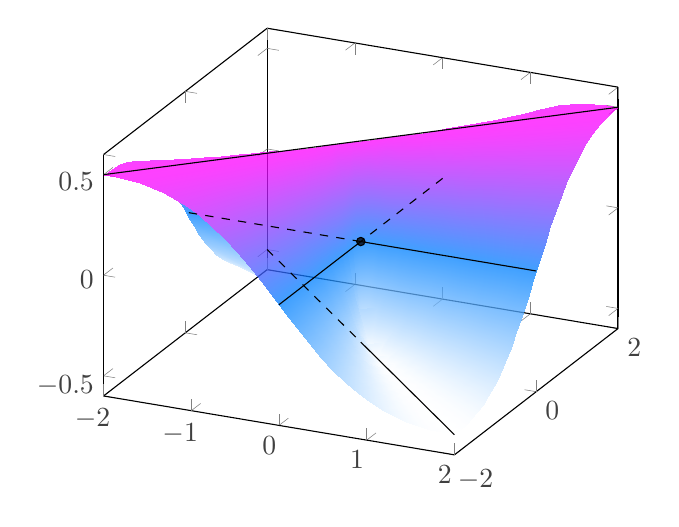
\begin{tikzpicture}
    \begin{axis}[%colormap/viridis,
    colormap/cool,
    height=7cm,
    surf, fill opacity=0.75,
    shader=flat,
    grid style=dashed,
    ]
    \addplot3[surf,domain=-2:2,samples=30, shader=interp] {x*y/(x*x + y*y)};
    \addplot3[domain=0:2, samples = 2, samples y=0] ({x}, {0}, {0});
    \addplot3[domain=0:2, samples = 2, samples y=0] ({0}, {-x}, {0});
    \addplot3[domain=-2:2, samples = 2, samples y=0] ({x}, {x}, {0.5});
    \addplot3[domain=0:2, samples = 2, samples y=0] ({x}, {-x}, {-0.5});
    \addplot3[domain=0:2, samples = 2, samples y=0, dashed] ({-x}, {x}, {-0.5});
    \addplot3[domain=0:-2, samples = 2, samples y=0, dashed] ({x}, {0}, {0});
    \addplot3[domain=0:-2, samples = 2, samples y=0, dashed] ({0}, {-x}, {0});
    \addplot3[mark=*, mark size=1.5] coordinates{(0,0,0)}; 
    \end{axis}
    \end{tikzpicture}
\end{center}


\end{example}
\end{remark}

\subsection{Eigenschaften von stetigen Funktionen}
\begin{satz}{Urbild von stetigen Funktionen}{urbild_stetige_fcns}
Seien $(X, d_X), (Y, d_Y)$ metrische Räume. Die Abbildung $f: X \to Y$ ist genau dann stetig, wenn für jede offene Teilmenge im Zielraum $Y' \subseteq Y$ auch das Urbild davon $f^{-1}(Y')$ offen ist:
$$f: X \to Y \text{ stetig} \iff \forall Y' \subseteq Y \text{ offen}: f^{-1}(Y') \text{ offen}$$

Es gilt äquivalent dazu auch die Aussage für abgeschlossene Mengen:
$$f: X \to Y \text{ stetig} \iff \forall Y' \subseteq Y \text{ abgeschlossen} \implies f^{-1}(Y') \text{ abgeschlossen}$$
\end{satz}
\begin{proof}
($\Longrightarrow$) Sei $f$ stetig und $Y' \subseteq Y$ offen und sei $x_0 \in X$ im Urbild $f^{-1}(Y')$, also $f(x_0) \in Y'$. Wir wollen nun zeigen, dass die Offenheit vom Urbild $f^{-1}(Y')$ gilt, also dass man für jedes $x_0$ eine $\delta$-Umgebung ($\subseteq X$) finden kann, welche komplett nach $Y'$ abgebildet wird. $Y'$ ist offen, also gibt es eine $\varepsilon$-Umgebung, sodass $B_\varepsilon(f(x_0)) \subseteq Y'$ gilt. Da $f$ stetig ist, können wir nun ein $\delta > 0$ wählen, sodass die gesamte $\delta$-Umgebung $B_\delta(x_0)$ nach $B_\varepsilon(f(x_0))$ abgebildet wird. Somit erhalten wir $B_\delta(x_0) \subseteq B_\varepsilon(f(x_0)) \subseteq Y'$, also die Behauptung.

($\Longleftarrow$) Sei nun das Urbild $f(Y') \subseteq X$ offen für alle offenen Teilmengen $Y' \subseteq Y$. Also gilt auch, dass für ein $\varepsilon > 0$ und ein $x_0 \in X$ die Menge $f^{-1}(B_\varepsilon(x_0)$ offen ist. Somit können wir eine $\delta$-Umgebung für $x_0$ wählen, sodass $B_\delta(x_0) \subseteq f^{-1}(B_\varepsilon(x_0)$, also die Stetigkeit $x \in B_\delta(x_0) \implies f(x) \in B_\varepsilon(f(x_0))$ gilt.

Die letzte Behauptung folgt direkt aus der Definition der Abgeschlossenheit: Falls $Y'$ abgeschlossen ist, ist das Komplement $(Y')^C$ offen. Zudem kann man sich schnell davon überzeugen, dass $f^{-1}(Y'^C) = (f^{-1}(Y'))^C$ gilt. Ersetzt man nun in den Beweisen oben $Y'$ mit $(Y')^C$ für geschlossene $Y'$, so erhält man die Behauptung.
\end{proof}

In anderen Worten können wir nun die Stetigkeit unabhängig von der Metrik und nur mit einer Topologie definieren: Nämlich sind Abbildungen stetig, falls das Urbild einer offenen Menge ebenfalls offen ist.

Diesen Satz können wir verwenden, um z.B. Aussagen über Lösungsmengen von Gleichungssystemen oder Ungleichungssystemen machen zu können:

\begin{example}[Offenheit von Lösungsmengen] Sei $X = \R^n$ und $L$ die Lösungsmenge einer stetigen, vektorwertigen Funktion $f: \R^n \to \R^m$ mit den Komponenten $x \mapsto (f_1(x_1,...,x_n), ..., f_m(x_1,...x_n))$:
$$ L = \setr{x \in \R^n }{ f(x)=0\quad \text{resp.}\quad \begin{matrix}f_1(x_1, ..., x_n) = 0\\ \vdots \\ f_m(x_1, ..., x_n) = 0 \end{matrix}}$$
Da alle $f_i$ mit $1 \leq i \leq n$ stetig sind und $L = f^{-1}(\{0\})$ das Urbild von der abgeschlossenen Menge $\{0\}$ ist, wissen wir aus dem Satz, dass auch $L$ abgeschlossen sein muss.

Analog dazu ist z.B. die Menge 
$$\setr{x \in \R^n }{ f(x)>0} = f^{-1}(\R_{>0})$$
offen, falls $f$ stetig ist.
\end{example}

Wir können mit dem obigen Satz \ref{satz:urbild_stetige_fcns} sehr elegant auch die Stetigkeit von Verknüpfungen stetiger Abbildungen zeigen:
\begin{satz}{Stetigkeit von Verknüpfungen}{}
Seien $(X, d_X), (Y, d_Y)$ und $(Z, d_Z)$ metrische Räume und $g: X \to Y, f: Y \to Z$ zwei stetige Abbildungen, dann ist auch die Verknüpfung $f \circ g : X \to Z$ stetig.
\end{satz}
\begin{proof}
Sei $Z'$ offen, dann gilt für das Urbild davon:
\begin{align*}
    (f\circ g)^{-1} &= \set{x \in X}{f(g(x)) \in Z'}\\
    &= \set{x \in X}{g(x) \in f^{-1}(Z')}\\
    &= g^{-1}(f^{-1}(Z'))
\end{align*}
Mit der Stetigkeit von $f$ und $g$  wissen wir, dass $f^{-1}(Z')$ offen und somit auch $g^{-1}(f^{-1}(Z'))$ offen ist. Nun folgt aus Satz \ref{satz:urbild_stetige_fcns}, dass die Verknüpfung $f\circ g$ stetig ist.
\end{proof}

\subsection{Beispiele zu Klassen von stetigen Funktionen}
Wir wollen nun die Stetigkeit von einigen Funktionen zeigen:

\begin{lemma}{konstante Funktion, Identität und Kehrwert}{}
\begin{enumerate}[label=(\alph*)]
    \item konstante Funktionen $f: X \to Y, x \mapsto a$ mit $a \in Y$
    \item Identität $id: X \to X, x \mapsto x$
    \item Kehrwert $(\:\cdot\:)^{-1}: K^\times \to K^\times, x \mapsto \frac{1}{x}$
\end{enumerate}
sind stetige Funktionen
\end{lemma}
\begin{proof}
Wähle für (a) $\delta$ beliebig, für (b) wähle $\delta = \varepsilon$ und für (c) wähle $\delta = \frac{1}{\varepsilon}$.
\end{proof}

\begin{lemma}{Addition und Multiplikation}{}
Die Addition und die Multiplikation $\R \times \R \to \R$ oder $\C \times \C \to \C$ sind stetig (mit der euklidischen Metrik).
\end{lemma}
\begin{proof} Wir wollen die Konvergenz von $+: \C^2 \to \C, (x,y) \mapsto x + y$ mittels der Folgenkonvergenz zeigen: Sei $(x_n,y_n)_n$ eine Folge in $\C^2$, die gegen $(x,y)$ konvergiert. Wir setzen diese in $+(x,y)$ ein und erhalten für das Stetigkeitskriterium:
\begin{align*}
    \abs{+(x_n,y_n) - +(x, y)} &= \abs{x_n - x + y_n - y}\\
    &\leq \abs{x_n-x} + \abs{y_n - y}\\
    &= \norm{(x_n-y_n) - (x,y)}_1 \longrightarrow 0 \quad (n \to \infty)
\end{align*}
Dabei haben wir im letzten Schritt die Konvergenz von  $(x_n,y_n)_n$ verwendet. Es folgt also, dass $\lim_{n \to \infty}(x_n + y_n) = x+y$ gilt. Analog wird die Stetigkeit für die Multiplikation gezeigt.
\end{proof}
Wir folgern aus diesem Lemma den allgemeineren Satz für die Stetigkeit von Linearkombinationen von Funktionen:
\begin{satz}{Summen, Produkte und Linearkombinationen}{}
Summen, Produkte und Linearkombinationen von Funktionen $X \to \R$ oder $\C$ sind stetig.
\end{satz}
\begin{proof}
Seien $f,g : X \to \C$ stetig, dann ist die Verknüpfung durch die Multiplikation $f \cdot g : X \to \C^2 \to \C$ gegeben durch
$$ x \mapsto (f(x), g(x)) \mapsto f(x) \cdot g(x)$$
wobei die erste Abbildung nach $\C^2$ wegen der Stetigkeit von vektorwertigen Funktionen (siehe Satz \ref{satz:stetigkeit_vektor_fcns}) stetig ist und die Stetigkeit von $\cdot$ im vorherigen Lemma gezeigt wurde. Insbesondere gilt das auch, wenn man $f(x) = a$ konstant wählt. Analog können wir das auch für die Addition von stetigen Funktionen zeigen. Durch Induktion können wir zeigen, dass auch Linearkombinationen aus stetigen Funktionen stetig sind.
\end{proof}
\begin{lemma}{Koordinatenabbildung/Projektionen}{}
Die Projektion $\pi_i : \R^n \to \R$ oder $\C^n \to \C$ mit $(x_1,...,x_n) \mapsto x$ ist stetig.
\end{lemma}
\begin{proof}
Wir verwenden für diesen Beweis die Notation $x = (x_1, ..., x_n)$ und $x_0 = (x_{0_1}, ..., x_{0_n})$. Sei $\varepsilon > 0$, dann erhalten wir für $\delta = \varepsilon$ mit $d(x, x_0) =    \norm{x-x_0}_2 < \delta$:
\begin{align*}
    \sqrt{\sum_{i=1}^n \abs{x_i - x_{0_1}}^2} &< \delta\\
    \abs{x_i - x_{0_i}} &< \varepsilon
\end{align*}
es folgt daraus die Stetigkeit von $\pi_i$:
$$d(\pi_i(x) , \pi_i(x_0)) = \abs{x_i - x_{0_i}} < \varepsilon$$
\end{proof}

\begin{lemma}{Lineare Abbildungen}{}
Lineare Abbildungen/Homomorphismen $\C^n \to \C^m \text{ oder } \R^n \to \R^m$ sind stetig.
\end{lemma}
\begin{proof} Da Linearkombinationen sowie die Koordinatenabbildung die Stetigkeit erhalten, können wir auch auf die Stetigkeit von linearen Endomorphismen schliessen: Sei $A$ eine lineare Abbildung
\begin{align*}
    A : \C^n &\to \C^m \text{ oder } \R^n \to \R^m\\
    x &\mapsto A(x)\\
    x_i &\mapsto  (a_{i1} \pi_1 + ... + a_{in} \pi_n)(x) \pi_n\\
    \begin{pmatrix} x_1\\\vdots\\x_n\end{pmatrix}&\mapsto\begin{pmatrix}a_{11} x_1 + ... + a_{1n} x_n\\\vdots\\a_{m1} x_m + ... + a_{mn}\end{pmatrix}
\end{align*}
wobei $a_{ij}$ die Koeffizienten der Matrix $[A]_\mathcal{B}$ bezüglich einer Basis $\mathcal{B}$ bezeichnet.
\end{proof}

\begin{lemma}{Polynomfunktionen}{}
Polynomfunktionen $P : \C^n \to \C$ sind stetig.
\end{lemma}
\begin{proof} Monome für vektorwertige Argumenten sind von der Form:
$$x = (x_1, ..., x_n) \mapsto x_1^{a_1}\cdot...\cdot x_n^{a_n}$$
wobei $a_i \in \N_0 = \{0,1,2,...\}$ die jeweiligen Potenzen bezeichnen. Da Monome Produkte von Projektionen $\pi_i$ sind, sind sie auch stetig. Polynome sind nun Linearkombinationen von Monomen, also folgt aus vorherigem Beispiel, dass Polynomfunktionen\footnote{Wir bezeichnen Polynomfunktionen umgangssprachlich häufig auch als ''Polynome'', wobei das Polynom erst durch das Einsetzen eines Arguments aus einem Ring entsteht.} ebenfalls stetig sind.
\end{proof}
\begin{example}Das Polynom $P: \C^3 \to \C$ mit $P(x,y,z) = x^2y + 3z$ ist stetig.\end{example}

\begin{satz}{Einschränkung von Abbildungen}{Einschraenkung_von_Abbildungen}
Seien $(X, d_X), (Y, d_Y)$ metrische Räume $X' \subseteq X$ eine Teilmenge und $f: X \to Y$ eine stetige Abbildung.

Die Einschränkung $f\vert_{X'} : X' \to Y$ ist stetig als Abbildung von $X' \to Y$.
\end{satz}
\begin{proof} $(X', d_X\vert_{X' \times X'})$ bildet einen metrischen Teilraum, wobei die offenen Mengen in $X'$ relativ offen sind in $X$. Sei nun $Y'$ eine offene Teilmenge in der Zielmenge $Y$, dann folgt für das Urbild der eingeschränkten Funktion:
\begin{align*}
    (f\vert_{X'})^{-1}(Y') &= \set{x \in X'}{f(x) \in Y'}\\
    &= f^{-1}(Y') \cap X'
\end{align*}
Aus der Stetigkeit von $f$ wissen wir, dass $f^{-1}(Y')$ offen ist. Also ist das Urbild relativ offen resp. offen als Teilmenge von $X'$, wobei aus Satz \ref{satz:urbild_stetige_fcns} folgt, dass $f\vert_{X'}$ stetig ist.
\end{proof}

\begin{lemma}{Rationale Funktionen}{}
Seien $P,Q$ Polynomfunktionen auf $\R^n \to \R$ und $D = \set{x \in \R^n}{Q(x) \neq 0}$ eine Teilmenge von $\R^n$ ohne den Nullstellen von $Q$, dann ist die rationale Funktion
$$f: D \to \R\text{ mit }f(x) = \frac{P(x)}{Q(x)}$$ stetig.
\end{lemma}
\begin{proof}
Wir erkennen, dass $D = Q^{-1}(\{0\})^C$ das Komplement von der abgeschlossenen Lösungsmenge $\set{x \in \R^n}{Q(x) = 0}$ ist, also $D$ folglich offen ist. $f$ ist die Multiplikation von $P(x)$ mit $\frac{1}{Q(x)}$ wobei $P$ und $Q$, die Multiplikation sowie der Kehrwert auf $Q(D) \subseteq X^\times$ stetig sind.
\end{proof} 

\begin{lemma}{Weitere stetige Funktionen}{}
\begin{itemize}
    \item Exponentialfunktion $\exp: \C \to \C$
    \item Trigonometrische Funktionen 
    \begin{itemize}
        \item $\sin, \cos: \C \to \C$
        \item $\tan: \C \setminus \set{x \in \C}{\cos(x) = 0} \to \C$
        \item $\arcsin, \arccos: [-1, 1] \to \R$
        \item $\arctan: \R \to \R$
    \end{itemize}
\end{itemize}
\end{lemma}

\section{Zusammenhang}
In $\R$ haben wir bereits den Begriff der Intervalle verwendet. Wir haben sie so charakterisiert, dass für jedes Paar von Punkten aus dem Intervall alle Punkte dazwischen ebenfalls im Intervall sind. Wir wollen davon nun den allgemeineren topologischen Begriff des Zusammenhangs definieren:
\begin{definition}{Zusammenhang}{}
Sei $(X, d)$ ein metrischer Raum, dann heisst $X$ \textbf{nicht zusammenhängend}, falls es zwei offene, nicht leere und disjunkte Teilmengen $U, V \subseteq X$ gibt, welche vereint $X$ ergeben:
$$X \text{ nicht zusammenhängend} \iff U \sqcup V = X$$
$X$ heisst \textbf{zusammenhängend}, falls für offene und disjunkte Teilmengen $U, V$ gilt:
$$X \text{ nicht zusammenhängend} \land U \sqcup V = X \iff V = \emptyset \lor U = \emptyset$$
\end{definition}
Wir haben in der Definition der Offenheit gesehen, dass jeweils die Menge $X$ und $\emptyset$ offene Mengen sind, welche gleichzeitig auf abgeschlossen sind, weil sie das Komplement voneinander sind. Diese Definition besagt nun, dass zusammenhängende metrische Räume nur genau diese zwei offenen \textbf{und} abgeschlossenen (\textbf{abgeschloffenen}) Mengen besitzen. Denn falls wir eine weitere solche Menge $U \neq X$ und $U \neq \emptyset$ hätten, so wäre das Komplement $U^C$ ebenfalls offen und abgeschlossen und $U \sqcup U^C = X$ wäre erfüllt.

\begin{example}
$X = (-\infty, 0) \cup (0, \infty) \subseteq \R$ wie auch $Y = [0,1] \cup \{2\}$ sind nicht zusammenhängend. Für $X$ können wir $U = (-\infty, 0)$ und $V = (0, \infty)$ wählen, für $Y$ analog $V' = [0,1]$ und $U' = \{2\}$. Man beachte, dass $V'$ und $U'$ als Teilmengen von $Y$ offen sind, auch wenn sie als abgeschlossene Mengen von $\R$ geschrieben sind.
\end{example}

Hingegen sind alle Intervalle $(a,b)$, $[a,b)$, etc. zusammenhängend. Wir sehen, dass das für $\R$ auch in die andere Richtung gilt:

\begin{satz}{Zusammenhängende Mengen auf $\R$}{zusammenhaengend_intervall_aufR}
Sei $A \subseteq \R$ eine Teilmenge, dann ist $A$ genau dann zusammenhängend, wenn es ein Intervall ist:
$$A \subseteq \R \text{ zusammenhängend} \iff A \text{ ist ein Intervall}$$
\end{satz}
\begin{proof}($\Longrightarrow$) Wir wollen diese Richtung mit der Kontraposition ''$A$ kein Intervall $\implies A$ nicht zusammenhängend'' beweisen. Da $A$ kein Intervall ist, gibt es für $a_1 < a_2 \in A$ ein $X \notin A$ mit $a_1 < x < a_2$ dazwischen. Wir konstruieren nun also die Mengen $U = (-\infty, x) \cap A$ und $V = (x, \infty) \cap A$. Überprüfen wir die Konditionen für eine nicht zusammenhängende Menge: $U,V$ sind relativ offen, das folgt aus der Definition der relativen Offenheit. Des Weiteren sind sie nicht leer, da $a_1 \in U$ und $a_2 \in V$ gilt. Auch sind $U,V$ disjunkt, da $U < V$, und es gilt $V \sqcup U = A$, da $x \notin A$ ist. Also ist $A$ keine zusammenhängende Menge.

($\Longleftarrow$) Wir nehmen an, dass $A$ ein nicht zusammenhängendes Intervall ist und führen es zu einem Widerspruch. Aus der Annahme wissen wir, dass disjunkte, nicht leere $U,V$ existieren, sodass $U \sqcup V = A$ gilt. Seien also $a_1 \in U$ und $a_2 \in V$ mit $a_1 < a_2$, dann können wir $x$ ''an der/einer Grenze'' wie folgt konstruieren:
$$x = \sup \set{y \in U}{[a_1, y] \subseteq U}$$
Mit dem Supremum ertasten wir also von $a_1$ aus die nächste rechte Grenze von $U$. $x$ wird zudem grössergleich $a_1$ sein per Definition des Supremums. Da $A$ per Annahme ein Intervall ist und $a_1 \leq x \leq a_2$ gilt, muss $x \in A$, also wegen $U \sqcup V = A$ entweder $x \in U$ oder $x \in V$ gelten. Beachte, dass das Supremum auch in $U \subseteq A$ liegen kann (i.e. das Maximum ist) und trotzdem noch (relativ) offen sein kann, weswegen wir beide Fälle betrachten müssen:

(Fall $x \in U$) Da $U$ offen ist, existiert ein $\varepsilon > 0$, sodass $B_\varepsilon(x) \in U$, also ist auch das Intervall $[x, x+\frac{\varepsilon}{2}]$ in $U$, was der Definition von $x$ widerspricht.

(Fall $x \in V$) Da $V$ offen ist, existiert ein $\varepsilon > 0$, sodass $B_\varepsilon(x) \in V$, also ist auch das Intervall $[x-\frac{\varepsilon}{2}, x]$ in $V$ und wegen der Disjunktheit nicht in $U$, welches auch ein Widerspruch zur Definition von $x$ ist.

Also ist $A$ zusammenhängend.
\end{proof}

Für stetige Abbildungen auf zusammenhängenden Mengen kann man sich nun vorstellen, dass das Bild davon ebenfalls zusammenhängend sein muss. Wir wollen daher folgenden Satz zeigen:

\begin{satz}{Abbildungen auf zusammenhängenden Mengen}{abb_auf_zusammenhaengenden_mengen}
Seien $(X,d_X), (Y, d_Y)$ zwei metrische Räume mit einer stetigen Abbildung $f : X \to Y$, dann gelten:
\begin{enumerate}[label=(\alph*)]
    \item Falls $X$ zusammenhängend und $f$ surjektiv\footnote{Ist nötig, da nicht getroffene Punkte vom Bild abgespalten sein könnten.} ist, dann ist auch $Y$ zusammenhängend.
    \item Falls $A \subseteq X$ zusammenhängend ist, dann ist auch das Bild $f(A) \subseteq Y$ zusammenhängend.
\end{enumerate}
\end{satz}
\begin{proof}
\begin{enumerate}[label=(\alph*)]
    \item Wir nehmen an, dass $Y$ nicht zusammenhängend ist, somit gibt es offene, nicht-leere und disjunkte $U, V \subseteq Y$, sodass für die Vereinigung $U \sqcup V = Y$ gilt. Da $f$ stetig ist, sind die Urbilder $\tilde{U} = f^{-1}(U) \subseteq X$ und $\tilde{V} = f^{-1}(V)$ offen als auch disjunkt, da $f^{-1}(U) \cap f^{-1}(V) = f^{-1}(U \cap V) = f^{-1}(\emptyset) = \emptyset$ gilt. Zudem wissen wir auch aufgrund der Surjektivität (und Wohldefiniertheit) von $f$, dass $\tilde{U} \sqcup \tilde{V} = X$ gelten muss, da $U \sqcup V = Y$ den gesamten Wertebereich abdeckt. Zudem sind $\tilde{U}$ und $\tilde{V}$ nicht leer, da $V$ und $U$ nicht leer sind und $f$ surjektiv ist. Also ist $X$ nicht zusammenhängend.
    \item folgt aus (a), weil $f\vert_A : A \to f(A) \subseteq Y$ gilt und $f$ auf sein Bild surjektiv ist.
\end{enumerate}
\end{proof}

Wir können aus dieser Erkenntnis den verallgemeinerten Zwischenwertsatz formulieren:
\begin{korollar}{verallgemeinerter Zwischenwertsatz}{}
Sei $X$ eine zusammenhängender metrischer Raum und $f: X \to \R$ eine stetige Funktion. Seien zudem $a,b \in X$, dann gibt es für jedes $y$ zwischen den Bildern $f(a)$ und $f(b)$ ein $x \in X$, sodass $f(x) = y$ gilt.
\end{korollar}
\begin{proof}
Das Bild $f(X)$ ist nach obigem Satz \ref{satz:abb_auf_zusammenhaengenden_mengen} (b) ebenfalls zusammenhängend. Da es eine zusammenhängende Menge auf $R$ ist, ist $f(X)$ zudem ein Intervall nach Satz \ref{satz:zusammenhaengend_intervall_aufR}, wodurch für alle Punkte zwischen $f(a)$ und $f(b)$ getroffen werden müssen.
\end{proof}

\subsection{Wegzusammenhang}
Wir haben den Begriff des Weges Ende letztes Semester eingeführt. Kurz gesagt ist es eine stetige Funktion zwischen zwei Punkten $a$ und $b$.

%\begin{definition}{Weg}{} ein \textbf{Weg} von $x \in X$ nach $y \in X$ ist eine stetige Abbildung $\gamma : [0, 1] \to X$, sodass $\gamma(0) = x$ und $\gamma(1) = y$.
%\end{definition}
\begin{definition}{Wegzusammenhang}{}
Wir nennen eine Menge $X$ \textbf{wegzusammenhängend}, falls es für alle $x,y \in X$ einen Weg von $x$ nach $y$ gibt.
\end{definition}
\begin{example}
Der $\R^n$ ist wegzusammenhängend: Seien $x,y \in \R^n$, dann ist $\gamma: [0,1] \to \R^n$ mit $t\mapsto x + t(y-x)$ ein Weg von $x$ nach $y$.

Hingegen ist $\R\setminus \{0\}$ nicht wegzusammenhängend, da aus dem Zwischenwertsatz folgt, dass jeder Weg z.B. von $-1$ nach $1$ durch $0$ gehen muss. $\R^n \setminus \{0\}$ mit $n\geq 2$ ist jedoch wieder wegzusammenhängend, da man einen Weg um die $0$ finden kann.
\end{example}

\begin{satz}{Wegzusammenhang und Zusammenhang}{Wegzusammenhang_und_Zusammenhang}
Falls $X$ eine wegzusammenhängende Menge ist, so ist $X$ auch zusammenhängend.

\centering $X$ wegzusammenhängend $\implies X$ zusammenhängend
\end{satz}
\begin{proof}
Sei $X$ wegzusammenhängend aber nicht zusammenhängend. Dann gibt es offene, nicht-leere und disjunkte $U, V \subseteq Y$, sodass für die Vereinigung $U \sqcup V = X$ gilt. Wähle nun $x \in U$ und $y \in V$, dann existiert wegen dem Wegzusammenhang ein Weg $\gamma$. Da $[0,1]$ zusammenhängend und $\gamma$ stetig ist, folgt aus Satz \ref{satz:abb_auf_zusammenhaengenden_mengen} (b), dass das Bild $A$ auch zusammenhängend ist. Da $A \subseteq X = U \sqcup V$ gilt, müsste auch $A = (U \cap A) \cup (V \cup A)$ gelten. Da Schnitte von offenen Mengen aber offen sind und $(U \cap A)$ resp. $(V \cap A)$ jeweils offen sind, kann $A$ nicht zusammenhängend sein, also ein Widerspruch.
\end{proof}

Wir können im folgenden Beispiel erkennen, dass der Wegzusammenhang eine stärkere Eigenschaft ist als der Zusammenhang selber:

\begin{example}\label{ex_topologists_curve}
Die Menge $T = \set{(x,\sin \frac{1}{x}) \in \R^2}{x \in \R_{\neq 0}} \cup \{(0,0)\}$\footnote{Mehr dazu unter \href{https://en.wikipedia.org/wiki/Topologist\%27s_sine_curve}{diesem} Link} ist zusammenhängend, denn jeder $\varepsilon$-Ball um $(0,0)$ schneidet sich mit dem Rest der Menge. Aber es lässt sich kein Weg zu $(0,0)$  oder von der linken Hälfte in die rechte Hälfte finden, da ein solcher Weg ''unendlich'' wäre.
\begin{figure}[hbt!]
    \centering
    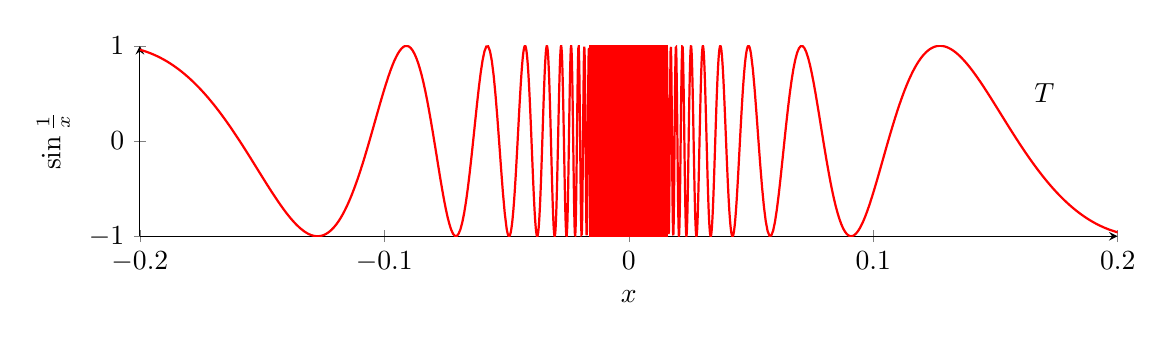
\begin{tikzpicture}
    \begin{axis}[
        axis lines = left,
        ytick={-1, 0, 1},
        xtick={-0.2, -0.1, 0, 0.1, 0.2},
        xlabel = $x$,
        ylabel = {$\sin \frac{1}{x}$},
        width=14cm,height=4cm,
    ]
    \addplot [domain=-0.05:-0.2, samples=200, color=red, style={thick}] {sin(deg(1/x))};
    \addplot [domain=-0.015:-0.05, samples=250, color=red, style={thick}] {sin(deg(1/x))};
    \addplot [domain=0.015:0.05, samples=250, color=red, style={thick}] {sin(deg(1/x))};
    \addplot [domain=0.05:0.2, samples=200, color=red, style={thick}] {sin(deg(1/x))};
    \addplot [fill, color=red] coordinates {(-0.016,1) (0.016,1) (0.016,-1)(-0.016,-1) } --cycle;
    \node at (axis cs:0.17,0.5) {$T$};
    \end{axis}
\end{tikzpicture}
\end{figure}
\end{example}
Unter einigen Einschränkungen können wir aber eine Äquivalenz formulieren:
\begin{satz}{(Weg)zusammenhang von offenen Teilmengen in $\C^n$}{}
Sei $U \subseteq \R^n$ oder $\C^n$ eine offene Teilmenge mit der euklidischen Metrik, dann gilt:
$$U \text{ zusammenhängend} \iff U \text{ wegzusammenhängend}$$
\end{satz}
Beachte hier genau, welches ''offen'' wir verwenden. Hier, im Gegensatz zur Definition des Zusammenhangs, reden wir wieder von offenen Teilmengen $\subseteq \R^n$ oder $\C^n$. Im vorherigen Beispiel \ref{ex_topologists_curve} konnten wir keine zwei offenen, disjunkte Teilmengen von $T$ finden, wobei $T$ als offen in sich selber gilt. $T$ als Teilmenge von $\R^2$ ist jedoch keine offene Menge.
\begin{proof}
($\Longrightarrow$) Sei $x_0$ ein Punkt aus $U$. Wir wollen nun für den Wegzusammenhang zeigen, dass es zu jedem Punkt aus $U$ einen Pfad zu $x_0$ gibt. Falls das erfüllt ist, kann auch ein Pfad zwischen zwei beliebigen Punkten gefunden werden. Wir definieren die Menge$$G = \set{x \in U}{\text{es existiert ein Pfad zu }x_0}$$ für welche Punkte es einen Pfad zu $x_0$ gibt. Wir wollen zeigen, dass $G$ offen und abgeschlossen ist, welches in einer zusammenhängenden Menge nach Definition bedeutet, dass $G = U$ gilt.

A priori wissen wir aber nur folgendes über diese Menge: Sie ist nicht leer, da wir für $x_0$ bereits den ''konstanten'' Pfad kennen. Sei also $x$ ein Element aus diesem nicht-leeren $G$ (notfalls $x_0$ selber), dann wissen wir aufgrund der Offenheit von $U$, dass ein $\varepsilon > 0$ existiert, sodass der Ball $B_\varepsilon(x)$ komplett in $U$ enthalten ist. Wir wollen zeigen, dass dieser Ball aber auch in $G$ liegt. Wir können von einem Punkt aus dem Ball $y \in B_\varepsilon(x)$  einen Pfad $\gamma_y$ zu $x$ finden, indem wir (\todo{was ist die Begründung?}). Da $x \in G$ ist, gibt es auch bereits einen Pfad $\gamma_x$ von $x_0$ zu $x$. Wir können diese nun wie folgt zusammensetzen:
$$\gamma(t) = \begin{cases} \gamma_x(2t) & 0 \geq t \geq \frac{1}{2} \\ \gamma_y(2t-1) & \frac{1}{2} \geq t \geq 1\end{cases}$$
Wir erkennen, dass der zusammengesetzte Pfad $\gamma$ auch tatsächlich stetig ist, da $\gamma_x(1) = \gamma_y(0) = x$ gilt. Also ist $y \in B_\varepsilon(x)$, wodurch $G$ offen ist.

Nun ist zu zeigen, dass $G$ auch abgeschlossen ist, also das Komplement $U \setminus G$ offen ist. Dies können wir analog mit Punkten zeigen, die keinen Pfad au $x_0$ haben, wodurch deren $\varepsilon$-Umgebung ebenfalls keinen Pfad zu $x_0$ haben kann. Wir schliessen daraus, dass $U\setminus G$ ebenfalls offen sein muss und, da $U$ zusammenhängend ist, gleich der leeren Menge sein muss. Somit sehen wir, dass $G = U$ gilt.

($\Longleftarrow$) Dies haben wir bereits im Allgemeinen gezeigt in Satz \ref{satz:Wegzusammenhang_und_Zusammenhang}
\end{proof}

Wir wollen noch einen interessanten topologischen Begriff einführen:
\begin{definition}{Homemorphie}{}
Zwei metrische Räume $X,Y$ heissen \textbf{homöomorph/homeomorph}, falls es eine bijektive stetige Funktion $f: X \to Y$ gibt, welche auch eine stetige Inverse $Y \to X$ besitzt.
\end{definition}
\begin{example} Wir können mit dem Begriff des Zusammenhangs zeigen, dass der Einheitskreis $S^1=\set{x \in \R^2}{\norm{x}_2 = 1}$ und die reellen Zahlen $\R$ nicht homeomorph sind:
\begin{proof}
Sei $f : S^1 \to \R$ eine homeomorphe Abbildung. Wähle ein beliebiges $x \in S^1$ und betrachte die Mengen $U = S^1 \setminus \{x\}$ und $V = \R \setminus \{f(x)\}$. Wir erkennen, dass $U$ nach wie vor zusammenhängend ist (\todo{Beweis}) und $V = (-\infty, f(x)) \cup (f(x), \infty)$ nicht mehr zusammenhängend ist. Da aber $f\vert_U: U \to V$ stetig ist (Satz \ref{satz:Einschraenkung_von_Abbildungen}) und stetige Funktionen auf zusammenhängenden Mengen ein zusammenhängendes Bild besitzen müssen (Satz \ref{satz:abb_auf_zusammenhaengenden_mengen}), erhalten wir einen Widerspruch, da $V$ nicht zusammenhängend sein kann.
\end{proof}
\end{example}

\section{Vollständige metrische Räume}
Wir haben die Existenz vom Supremum resp. die Konvergenz von Cauchy-Folgen als Kriterium verwendet, um die Vollständigkeit zu charakterisieren. Wir möchten nun nochmals dieselben Begriffe mit dem topologischen Hintergrund definieren.

\begin{definition}{Cauchy-Folge}{}
Sei $(X,d)$ ein metrischer Raum, dann ist eine Folge $(x_n)_{n \in \N}$ in $X$ eine \textbf{Cauchy-Folge}, falls zu jedem $\varepsilon >0$ ein $n_0 \in \N$ existiert, sodass
$$n,m \geq n_0 \implies d(x_n, x_m) < \varepsilon$$
\end{definition}
Die einzige Änderung an dieser Definition ist die Verwendung der Metrik anstelle der Betragsfunktion.

Der Vorteil von dieser Definition ist, dass wir den Grenzwert nicht zu wissen brauchen, um eine Aussage über die Konvergenz einer Folge machen zu können. Denn wir haben konvergente Folgen so definiert, dass die Differenz zum Grenzwert beliebig klein gemacht werden kann resp. dass der Grenzwert der Limes der Folge ist. Mit dem Cauchy-Kriterium können wir also ohne Limes und Grenzwert zeigen, dass eine Folge cauchy ist und somit neue Objekte, z.B. $\pi$ oder $e$ definieren.

\begin{lemma}{}{}
Jede konvergente Folge ist eine Cauchy-Folge:
\begin{gather*}
    \exists x: \forall \varepsilon >0\ \exists n_0 \in \N: n \leq n_0 \implies d(x, x_n) < \varepsilon \\ \big\Downarrow \\ \forall \varepsilon >0\ \exists n_0 \in \N: n,m \geq n_0 \implies d(x_n, x_m) < \varepsilon
\end{gather*}
\end{lemma}
\begin{proof}
Sei $x = \lim_{n \to \infty} x_n$ der Grenzwert der Folge $(x_n)_{n\in \N}$. Dann gibt es für ein $\varepsilon > 0$ ein $n_0$, sodass $d(x_n,x) < \frac{\varepsilon}{2}$ für alle $ n \geq n_0$ gilt. Daraus folgt für alle $n,m \geq n_0$:
\begin{align*}
    d(x_n,x_m) &\leq d(x_n,x) + d(x,x_m)\\
    &\leq d(x, x_n) + d(x, x_m)\\
    &\leq \frac{\varepsilon}{2} + \frac{\varepsilon}{2} = \varepsilon
\end{align*}
\end{proof}
Die umgekehrte Implikation, dass jede Cauchy-Folge auch konvergiert, gilt jedoch nicht im Allgemeinen. Falls das jedoch in einem Raum gilt, so nennen wir diesen \textbf{vollständig}:

\begin{definition}{Vollständigkeit}{}
Ein metrischer Raum $X$ heisst \textbf{vollständig}, falls alle Cauchy-Folgen in $X$ konvergieren.
\end{definition}
Wir wissen bereits, dass $\R$ vollständig ist, also können wir diesen Satz formulieren:
\begin{satz}{Vollständigkeit von $\R^N$ und $\C^N$}{}
$\R^N$ mit der euklidischen Metrik ist vollständig für alle $N \geq 1$.

Daraus folgt auch die Vollständigkeit von $\C^N \cong \R^{2N}$.
\end{satz}
\begin{proof} Wir verwenden Stetigkeit und Linearität der Projektionen $\pi_i: \R^N \to \R$, $(x_1, ..., x_n) \mapsto x_i$, u.a. auch um Doppelindeces zu vermeiden. Wir erkennen, dass im allgemeinen
$$\abs{\pi_i(x)} \leq \sqrt{x_1^2+...+x_N^2} = \norm{x}_2$$
gilt. Sei nun $(x_n)_{n \in \N}$ eine Cauchy-Folge mit $x_n \in \R^N$. Für das $n$-te Folgenglied gilt also $x_n = (\pi_1(x_n),..., \pi_N(x_n)) \in \R^N$. Da $(x_n)_{n \in \N}$ eine Cauchy-Folge ist, gilt für $n,m \in \N$
$$\abs{\pi_i(x_n) - \pi_i(x_m)} = \abs{\pi_i(x_n-x_m)} \leq \norm{x_n - x_m}_2$$
Somit ist auch die Folge der Projektionen $(\pi_i(x_n))_{n \in x}$ eine Cauchy-Folge in $\R$ für jede Dimension $i = 1,...,N$. Also existiert für jedes $i$ ein Grenzwert $y_i = \lim_{n \to \infty} \pi_i(x_n)$, da wir wissen, dass Cauchy-Folgen in $\R$ konvergieren.

Wir wollen nun zeigen, dass $y = (y_1,...,y_N) \in R^N$ der Grenzwert $\lim_{n \to \infty}x_n$ der ursprünglichen Folge ist. Wir finden für die Distanz zwischen einem Folgenglied $x_n$ und $y$ den Ausdruck
$$d(x_n, y) = \sqrt{\sum_{i = 1}^N \abs{\pi_i(x_n) - y_i}^2}$$
welcher beliebig klein gemacht werden kann, da alle Terme der Summe nach $0$ gehen. Also ist $\R^N$ ebenfalls vollständig.
\end{proof}
\begin{satz}{Vollständigkeit von abgeschlossenen Teilmengen}{Vollstaendigkeit_abgeschlossene_Teilmengen}
Abgeschlossene Teilmengen von vollständigen metrischen Räumen sind als metrische Teilräume ebenfalls vollständig.
\end{satz}
\begin{proof}
Übungsserie 3
Idee: Charakterisierung einer abgeschlossenen Menge: genau dann abgeschossen, wenn der Grenzwert einer konvergenten Folge in der Teilmenge liegt.
\end{proof}

\begin{example}
$[a, b] \subseteq \R$ ist vollständig, jedoch ist $(0,1]$ nicht vollständig, da die Cauchy-Folge $(\frac{1}{n})_{n \in \N}$ ihre Elemte in $(0,1]$ hat, aber nicht als Folge des metrischen Teilraums $(0,1]$ konvergiert.
\end{example}

\subsection{Klassen von Beispielen}
Hier einige Beispiele von vollständigen Mengen 
\begin{enumerate}
    \item abgeschlossene Teilmengen $A \subseteq \R^N$
    \item $C(K)$ stetige Funktionen auf einem kompakten Intervall $K = [a,b]$
\end{enumerate}
\begin{proof}
Siehe allgemeineren Beweis für beliebige kompakte metrische Räume \todo{ref Beweis}
\end{proof}

\begin{remark}
Falls $X$ ein normierter Vetorraum mit der induzierten Metrik $d(x,y) = \norm{x-y}$ ist und $\Nrm'$ eine zu $\Nrm$ äquivalente Norm ist (siehe Definition in Abschnitt \ref{cha_eq_norms}), dann sind Cauchy-Folgen bezüglich $\Nrm$ auch Cauchy-Folgen bezüglich $\Nrm'$:
$$\norm{x_n-x_m} < \varepsilon \implies \norm{x_n-x_m}' \leq c_2 \varepsilon$$
wobei wegen der Äquivalenz der Normen $c_1 \norm{x} \leq \norm{x}' < c_2 \norm{x}$ gilt. 
\end{remark}

\subsection{\textsc{Banach}'scher Fixpunktsatz}
Nehmen wir eine Weltkarte, welches eine skalierte und gestreckte Version der realen Welt ist, dann gibt es unabhängig von der Orientation der Karte immer einen Punkt darauf, der genau über dem Punkt in der realen Welt liegt, den er abbildet/auf der Karte bezeichnet. Es ist also ein \textbf{Fixpunkt}, der durch die Abbildung von der realen Welt auf die Karte nicht verschoben hat.

Wir wollen diese Eigenschaft nun topologisch in Formeln fassen. Hierfür wollen wir zuerst einige Begriffe einführen:

\begin{definition}{Fixpunkt}{}
Sei $f: X \to X$ eine (Selbst)abbildung, dann heisst $x \in X$ ein Fixpunkt, falls $f(x) =x$ gilt.
\end{definition}

Auf einem Funktionsgraphen sind die Fixpunkte einer Funktion die Projektion der Schnittpunkte zwischen der Funktion und der Geraden $x = y$ auf die $x$-Achse.
\begin{example}
Der Goldene Schnitt $\varphi = \frac{1+\sqrt{5}}{2}$ und $\psi = \frac{1-\sqrt{5}}{2}$ Fixpunkte der Funktion $1 + \frac{1}{x}$.
\begin{figure}[hbt!]
    \centering
    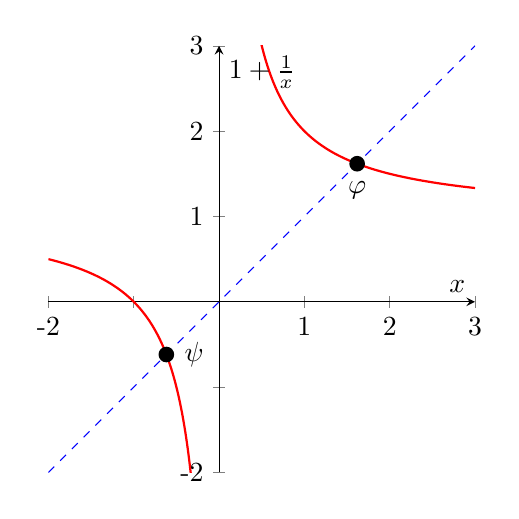
\begin{tikzpicture}
    \begin{axis}[
        axis lines = center,
        xlabel = $x$,
        ylabel = {$1 + \frac{1}{x}$},
        ytick = {-2,-1,1,2,3},
        xtick = {-2,-1,1,2,3},
        xmin=-2,xmax=3,ymin=-2,ymax=3,
        width=7cm,height=7cm,
        xticklabels={-2,,1,2,3},
        yticklabels={-2,,1,2,3},
    ]
    \addplot [domain=-2:-0.3, samples=200, color=red, style={thick}] {1+(1/x)};
    \addplot [domain=0.4:3, samples=200, color=red, style={thick}] {1+(1/x)};
    \addplot [domain=-2:3, samples=5, color=blue, dashed] {x};
    \node[label={270:{$\varphi$}},circle,fill,inner sep=2pt] at (axis cs:1.618,1.618) {};
    \node[label={0:{$\psi$}},circle,fill,inner sep=2pt] at (axis cs:-0.618,-0.618) {};
    \end{axis}
\end{tikzpicture}
\end{figure}
\end{example}

Wir wollen und nun die Frage stellen, wie man solche Fixpunkte findet. Man könnte sie versuchen, iterativ vorzugehen: Man beginnt mit einem $x_0 \in X$ und definiert $x_{n+1}$ rekursiv durch $x_{n+1} = f(x)$ für $n \geq 1$. Falls die Folge $(x_n)$ konvergiert mit dem Grenzwert $x = \lim_{n \to \infty}$, dann gilt 
\begin{align}\label{eq_fixpunkt}
    f(x) = \lim_{n \to \infty} f(x_n) = \lim_{n \to \infty} x_{n+1} = x    
\end{align}

\begin{example} Also ist $\varphi = 1+\frac{1}{1+\frac{1}{1+...}}$ ein Fixpunkt.
\end{example} 

Man kann mit dieser Methodik auch Gleichungen $g(x) = 0$ lösen. Die Stetigkeit von $g(x)$ ist dabei notwendig, da wir einen Grenzwert bilden.
\begin{enumerate}
    \item Schreibe die Gleichung als Fixpunktgleichung mit $x = f(x)$, also z.B. $f(x) = x+g(x)$
    \item Wähle einen Anfangswert $x_0$ und definiere $x_{n+1} = f(x_n)$
    \item Man ''hofft'', dass die Folge $(x_n)$ konvergiert. Wenn diese Folge konvergiert, wird der Grenzwert ein Fixpunkt sein.
\end{enumerate}

Newton hat diesen Such-Algorithmus mit der Verwendung der Ableitung verbessert. Die durch $f(x) = x - \frac{g(x)}{g'(x)}$ definierte Folge konvergiert, falls das initiale $x_0$ nahe genug an einem Fixpunkt ist.

Wir können mit solchen Suchalgorithmen Fixpunkte finden, jedoch wollen wir mithilfe der Vollständigkeit eine allgemeine Aussage über Fixpunkte machen können. Wir Wollen, wie im Beispiel der Karte am Anfang des Abschnittes einen Begriff haben, für stetige ''verkleinernede'' Abbildungen haben:

\begin{definition}{Lipschitz-Kontraktion}{}
Sei $(X, d)$ ein metrischer Raum, dann ist eine Abbildung $f: X \to X$ eine \textbf{Lipschitz-Kontraktion}, wenn es eine Konstante $L \in [0, 1)$ gibt, so dass
$$d(f(x), f(x')) \leq L \cdot d(x,x')$$
für alle Punkte $x, x' \in X$ gilt. Lipsitz-Kontraktionen sind Lipschitz-stetig.
\end{definition}
\begin{proof}
Verwende $L$ als Lipschitz-Konstante. Man erhält direkt per Definition einer Lipschitz-Kontraktion $d(f(x), f(x')) \leq L \cdot d(x,x')$, das die Lipschitz-Stetigkeit zeigt.
\end{proof}
Nun können wir den \textsc{Banach}'schen Fixpunktsatz formulieren:
\begin{satz}{\textsc{Banach}'scher Fixpunktsatz}{}
Sei $f: X \to X$ eine Lipschitz-Kontraktion eines vollständigen metrischen Raums $X$, dann hat $f$ einen eindeutigen Fixpunkt $x\in X$.
\end{satz}
Mit diesem Satz werden später auch zeigen können, dass Differentialgleichungen immer eine Lösung haben.
\begin{proof}
(Existenz) Wir wählen ein $x_0 \in X$ und konstruieren eine Folge $(x_n)_{n \in \N}$ mit Gliedern $x_n = f^{\circ n}(x_0) = f\circ f...\circ f (x_0)$ also $x_{n+1} = f(x_n)$. Wir wollen zeigen, dass die Folge $(x_n)_{n \in \N}$ cauchy ist. Da Lipschitz-Kontraktionen stetig sind folgt daraus, dass die Folge konvergiert und der Grenzwert davon nach der Erkenntnis \ref{eq_fixpunkt} oben ein Fixpunkt ist. Wir betrachten nun also $d(x_n,x_m)$ zuerst für $m=n+1$:
\begin{align*}
    d(x_n,x_{n+1}) &= d(f(x_{n-1}), f(x_n))\\
    &\leq L \cdot d(x_{n-1}, x_n)\\
    &\leq L^n \cdot d(x_0, f(x_0))
\end{align*}
wobei wir beim letzten Schritt induktiv vorgegangen sind. $L^n$ wird für $L \in [0,1)$ beliebig klein, jedoch benötigen wir für Cauchy-Folgen die Aussage für ein $n$ und $m$. Sei also $n < m$, dann gilt:
\begin{align*}
    d(x_n,x_m) &\leq d(x_n, x_{n+1}) + d(x_{n+1}, x_{n+2}) + ... + d(x_{m-1}, x_m)\\
    &\leq (L^n + L^{n+1} + ... + L^{m-1}) \cdot d(x_0, f(x_0))\\
    &\leq (L^n + L^{n+1} + L^{n+2} + ...) \cdot d(x_0, f(x_0))\\
    &\leq \frac{L^n}{1-L} \cdot d(x_0, f(x_0)) \longrightarrow 0 \quad (n \to \infty)
\end{align*}
Wir können nun die Cauchy-Eigenschaft zeigen: Sei $\varepsilon > 0$ beliebig, dann können wir ein $n_0$ finden, sodass für $n_0 \leq n \leq m$ gilt:
$$d(x_n, x_m) \leq \frac{L^n}{1-L} \cdot d(x_0, f(x_0)) < \varepsilon$$
Der Fall $m = n$ ist trivial, da $d(x_n, x_n) = 0 < \varepsilon$ per Definition einer Metrik gilt. Da Metriken zudem symmetrisch sind, also $d(x_n, x_m) = d(x_m, x_n)$, gilt die Aussage für beliebige $n,m \geq n_0$, also ist die Folge eine Cauchy-Folge und der Grenzwert resp. der Fixpunkt existiert.

(Eindeutigkeit) Seien nun $x$ und $x'$ zwei Fixpunkte, dann gilt
\begin{align*}
    d(x,x') &= d(f(x), f(x'))\\
    &\leq L \cdot d(x, x')\\
    \underbrace{(1-L)}_{\leq 0}\cdot \underbrace{ d(x, x')}_{\geq 0} &\leq 0
\end{align*}
Diese letzte Ungleichung ist nur dann möglich, wenn $d(x,x') =0$, also $x = x'$ gilt.
\end{proof}

\subsection{Markow-Ketten und Wahrscheinlichkeitsmatrizen}
Wir möchten nun den \textsc{Banach}'schen Fixpunktsatz für das folgende Problem anwenden:

Wir haben System mit $N$ verschiedenen Zuständen und einen Begriff von Zeitschritten, wobei wir in jedem Schritt zufällig entscheiden, welchen nächsten Zustand wir annehmen (z.B. ''Random-Walk'' auf einem Schachbrett). Dies gibt uns eine Wahrscheinlichkeitsverteilung der Zustände, welche gegeben ist durch die Werte $x_1, ..., x_N$. Da es sich um Wahrscheinlichkeiten handelt, ist jedes $x_i$ positiv und die Summe aller $x_i$ ist immer 1: $\sum_{i=1}^N x_1 = 1$. Wir können also die Wahrscheinlichkeitsverteilung auch als Vektor im $R^N$ darstellen.

\begin{definition}{$(N-1)$ Simplex}{}
Wir nennen die Menge aller Vektoren aus $\R^N$ mit positiven Einträgen und $\Nrm_1 = 1$ den \textbf{$(N-1)$-Simplex}:
$$X = \set{x \in \R^N}{\forall i: x_i \geq 0, \sum_{i=1}^N x_i = 1}$$
$X$ ist also die Menge aller Wahrscheinlichkeitsverteilungen. Zudem ist $X$ eine abgeschlossene und vollständige Menge. 
\end{definition}
\begin{proof}
Wir bemerken, dass $X$ als Schnitt zwischen der Lösungsmenge $$L = \set{\R^N}{\norm{x}_1 = 1}$$ und dem rein positiven ''Quadranten'' von $\R^N_{x_i \geq 0}$ definiert ist. Da die Bedingung für $L$ eine Gleichung ist, gilt nach Satz \ref{satz:urbild_stetige_fcns}, dass $L$ abgeschlossen ist. Der Schnitt aus zwei abgeschlossenen Mengen ist ebenfalls abgeschlossen, also ist $X = L \cap \R^N_{x_i \geq 0}$ abgeschlossen.

Die Vollständigkeit von $X$ folgt aus Satz \ref{satz:Vollstaendigkeit_abgeschlossene_Teilmengen}.
\end{proof}

Nun können wir also die Wahrscheinlichkeit aller Zustände als Vektor eines $(N-1)$-Simplex' ausdrücken. Am Anfang eines Random-Walks wäre also der Eintrag des Startfeldes gleich $1$ und die restlichen gleich 0.

Wenn wir nun die Wahrscheinlichkeit, um in einem beliebigen Zeitschritt $(t \to t+1)$ vom Zustand $j$ in Zustand $i$ zu gelangen mit $p_{ij} \in [0,1]$ bezeichnen, dann gilt für die Wahrscheinlichkeit vom Zustand $i$:
$$x_i' = \sum_{j=1}^N p_{ij}$$
Wir können das auch als Skalarprodukt mit dem Vektor $x_i' = (p_{i1}, ..., p_{iN})\cdot x$ bezeichnen resp. kann man durch Matrixmultiplikation mit der \textbf{Wahrscheinlichkeitsmatrix} $P$ den Wahrscheinlichkeitsvektor $x'$ nach einer beliebigen Verteilung $x$ berechnen.
\begin{definition}{Wahrscheinlichkeitsmatrix}{}
Seien $p_{ij}$ \textbf{Übergangswahrscheinlichkeiten}, um vom Zustand $j$ in Zustand $i$ zu wechseln, dann ist
$$P = \big(p_{ij}\big)_{\substack{1 \leq i \leq N\\1 \leq j \leq N}} = \begin{pmatrix}
p_{11} & p_{12} & \cdots & p_{1N}\\
p_{21} & p_{22} & \cdots & p_{2N}\\
\vdots & \vdots & \ddots & \vdots\\
p_{N1} & p_{N2} & \cdots & p_{NN}
\end{pmatrix}
$$
die \textbf{Wahrscheinlichkeitsmatrix}. Es gilt $p_{ij} > 0 \forall i,j$ und $\sum_{i = 1}^N p_{ij} = 1$.
\end{definition}
Also gilt $$Px = \big(p_{ij}\big)_{\substack{1 \leq i \leq N\\1 \leq j \leq N}} x = x'$$
Betrachten wir $P$ also als Abbildung in $X$:
$$\norm{Px}_1 = \sum_{i=0}^N\sum_{j=0}^N p_{ij} x_j =  \sum_{j=0}^N x_j\left(\sum_{i=0}^N p_{ij}\right) = \sum_{j=0}^N x_j = 1$$
Wir erkennen, dass $P$ eine in $X$ abgeschlossene Abbildung $P: X \to X, x \mapsto Px$ auf der vollständigen Menge $X$ ist, also können wir den Langzeitverlauf $\lim_{n \to \infty} P^nx$ dieser stochastischen Dynamik betrachten. Wahrscheinlichkeitsmatrizen sind zudem Lipschitz-Kontraktionen für $\Nrm_1$:
$$\norm{Px-Px'}_1 \leq L \norm{x-x'}_1$$
mit $L= 1- \min\{p_ij\} < 1$ Aus der Abgeschlossenheit und der Vollständigkeit von $X$ und dem Banach'schen Fixpunktsatz lässt sich also ein eindeutiger Fixpunkt $x \in X$ finden. $x$ ist eine ''stationäre Verteilung'', also eine Wahrscheinlichkeitsverteilung, die invariant unter einem Zeitschritt ist. Aus Banach folgt, dass jeder beliebige Punkt aus $X$ zu diesem Fixpunkt konvergiert, also $\forall x_0 \in X$ gilt:
$$x = \lim_{n \to \infty} P^nx_0$$
Der Beweis, dass $P$ eine Lipschitz-Kontration ist, ist im Skript zu finden.

\begin{example}[Biased Coin]
Sei $p$ die Wahrscheinlichkeit von Zustand $1$ zu $2$ zu wechseln und $q$ für $2 \to 1$. Für die Übergangsmatrix erhalten wir:
$$P = \begin{pmatrix}
1-p & q \\ p & 1-q
\end{pmatrix}$$
Für die ersten beiden Schritte $P^0x_0$ und $P^1x_0$
$$x_0 = \binom{1}{0}, \quad x_1 = \binom{1-p}{p}$$
Im Unendlichen erhalten wir die Gleichgewichtsverteilung
$$x = \lim_{n \to \infty}P^nx_0 = \binom{\frac{q}{p+q}}{\frac{q}{p+q}}$$
\end{example}

\section{Kompakte metrische Räume}
Wir haben bereits in $\R$ gesehen, dass sich mit der Kompaktheit einer Menge sehr viele Aussagen machen lassen können. Wir wollen diesen Begriff daher auch Topologisch einführen\footnote{Siehe Skript für weitere Definitionen und Begriffe. Diese Einführung beruht auf Königsberger Analysis 2, Seiten 1-44.}. Wir werden folgende Begriffe verwenden:

\begin{definition}{Überdeckung \& Teilüberdeckung}{}
Sei $(X, d)$ ein metrischer Raum und $Y \subseteq X$ eine Teilmenge. Eine offene \textbf{Überdeckung} von $Y$ ist eine Menge $\mathcal{U}$ von offenen Teilmengen, die $Y$ überdecken, d.h. $\forall y \in Y \exists U \in \mathcal{U}$, sodass $y \in U$ gilt.
$$Y \subseteq \bigcup_{U \in \mathcal{U}}$$

Eine \textbf{Teilüberdeckung} von $\mathcal{U}$ ist eine Teilmenge von $\mathcal{U}$, die immer noch eine offene Überdeckung von $Y$ ist.
\end{definition}
Nun kommen wir zur topologischen Definition der Kompaktheit:
\begin{definition}{Kompaktheit/Überdeckungskompaktheit}{}
Eine Teilmenge $Y \subseteq X$ ist \textbf{kompakt}, falls jede offene Überdeckung eine endliche Teilüberdeckung besitzt:
$$\forall \mathcal{U} \text{ offene Überdeckung: } \exists U_1, ..., U_n \subseteq \mathcal{U}: Y \subseteq \bigcup_{i = 1}^n U_i $$
\end{definition}
In Worte gefasst können wir aus \textit{jeder} offenen Überdeckung von $Y$ \textit{endlich} viele Mengen $U_i$ wählen, welche vereint immer noch $Y$ enthalten.

\begin{example}
$\mathcal{U} = \set{U_n}{n \in \Z}$ mit $U_n = (n-1, n+1)$ ist eine offene Überdeckung von $\R$, jedoch gibt es keine endliche Teilüberdeckung in $\mathcal{U}$.

$\mathcal{U}$ enthält für eine abgeschlossene Menge $[a,b] \subseteq \R$ eine endliche Teilüberdeckung, z.B. $\set{U_n}{n \in [a, b]} \subseteq \mathcal{U}$. Dies ist jedoch kein Beweis, da wir das für alle Überdeckungen zeigen müssten.
\end{example}

\begin{lemma}{Kompaktheit der Referenzmenge}{}
Die Menge $X$ heisst kompakt, falls $X$ als Teilmenge von sich selbst kompakt ist.
$$\forall \mathcal{U} \text{ offene Überdeckung: } \exists U_1, ..., U_n \subseteq \mathcal{U}: X \subseteq \bigcup_{i = 1}^n U_i $$
\end{lemma}
\begin{remark}
Man kann mit diesem Lemma die Kompaktheit eines Teilraums $Y \subseteq X$ auch formulieren, ohne den ''Mutterraum'' $X$ betrachten zu müssen. Denn offene Mengen in $Y$ sind relativ offene Mengen in $X$, also kann man eine Überdeckung von $Y$ auch auf $X$ erweitern, resp. von $X$ auf $Y$ einschränken und dieselbe Aussage über die Kompaktheit machen.
\end{remark}

\begin{example}[Wichtiges Beispiel]
$[a,b] \subseteq \R$ ist kompakt, allgemeiner sind Quader $[a_1, b_1] \times ... \times [a_n, b_n] \subseteq \R^n$ kompakt.
\begin{proof}[Heine-Borell]
(für Würfel in $n$ Dimensionen) Sei $W = [-\frac{L}{2}, \frac{L}{2}]^n \subseteq \R^n$ und $\mathcal{U}$ eine offene Überdeckung von $W$. Wir nehmen an, dass es keine endliche Teilüberdeckung von $\mathcal{U}$ gibt, die $W$ überdeckt und wollen es zum Widerspruch führen. Wir teilen also $W$ in $2^n$ Würfel mit halber Seitenlänge. Da es keine komplette Teilüberdeckung gibt, muss daher mindestens einer dieser $2^n$ Würfel keine Überdeckung haben (ansonsten würde die Vereinigung $W$ überdecken). \todo{Beweis verstehen}

Also muss mindestens ein Würfel $W_i$ mit Seitenlänge $L\cdot 2^{-i}$ keine Teilüberdeckung haben.

Maximale Distanz zwischen zwei Punkten (in $\Nrm_2$) ist $\sqrt[2]{n} \cdot ...$
\end{proof}

(Gegenbeispiel) Sei $(0 ,1] \subseteq \R$, dann ist auch $U_j = (\frac{1}{j}, \infty)$ mit $\set{U_j}{j\in \N}$, eine offene Überdeckung von $(0,1]$, jedoch gibt es keine endliche Teilüberdeckung.
\end{example}

Wir können eine weitere Art von Kompaktheit definieren:
\begin{definition}{Folgenkompaktheit/Bolzano-Weierstrass Kompaktheit}{}
Ein metrischer Raum $(X, d)$ heisst \textbf{folgenkompakt}, falls jede Folge in $X$ eine in $X$ konvergente Teilfolge besitzt.
\end{definition}
Alternativ kann man auch sagen, dass die Menge der Punkte jeder Folge $M = \set{x_i}{i \in \N}$ einen Häufungspunkt $x \in X$ besitzt:
$$\forall \varepsilon > 0: B_\varepsilon(x) \cap M \neq \emptyset$$

Im Allgemeinen gilt die Äquivalenz von Folgenkompaktheit und Überdeckungskompaktheit nicht, jedoch gilt sie, wie wir im nächsten Abschnitt sehen werden, in allen metrischen Räumen.

\subsection{Eigenschaften von kompakten Mengen}

Wir haben einige Eigenschaften von stetigen Funktionen auf kompakten Mengen gesehen: Sie nehmen ihr Minimum resp. Maximum an, sie sind begrenzt, sie sind Lipschitz-stetig, etc...

\begin{lemma}{Kompaktheit $\implies$ Folgenkompaktheit}{kompaktheit_folgkmpkt}
Sei $X$ ein kompakter metrischer Raum, dann ist $X$ folgenkompakt.
\end{lemma}
\begin{remark}
Die Umkehrung gilt auch, jedoch werden wir diese in \ref{satz:heine_borel} nur für $\R^n$ zeigen.
\end{remark}
\begin{proof}
Sei $X$ kompakt und $(x_n)_{n \in \N}$ eine Folge in $X$. Nehmen wir nun an, dass $(x_n)_{n \in \N}$ \textit{keine} konvergente Teilfolge besitzt, also dass es keinen Grenzwert $x \in X$ gibt. Also darf es für jeden Punkt $x \in X$ nur endlich viele Folgenglieder geben, die in der $\varepsilon_x$-Umgebung liegen: $\abs{\set{x_n}{x_n \in B_{\varepsilon_x}, n \in \N}} < \infty$. Wir bilden nun die Überdeckung $\mathcal{U} = \set{B_{\varepsilon_x}}{x \in X}$. Da $X$ kompakt ist, wissen wir auch, dass es eine endliche Teilüberdeckung $B_{\varepsilon_1}(y_1),..., B_{\varepsilon_n}(y_n) \in \mathcal{U}$ mit $B_{\varepsilon_1}(y_1) \cup ... \cup B_{\varepsilon_n}(y_n) = X$ gibt. Für die Folge bedeutet das aus der Konstruktion, dass nur endlich viele Folgenglieder in $X$ liegen können, also ein Widerspruch.
\end{proof}

\begin{definition}{Beschränktheit}{}
Der Teilraum $A \subseteq X$ heisst \textbf{beschränkt}, wenn ein Punkt $a \in X$ und ein Radius $r > 0$ existieren, sodass $A \subseteq B_r(a)$ gilt.
\end{definition}

\begin{lemma}{Folgenkompaktheit $\implies$ Abgeschlossenheit}{folgkmpkt_abgeschl}
Sei die Teilmenge $A \subseteq X$ folgenkompakt, dann ist $A$ abgeschlossen und beschränkt.
\end{lemma}

\begin{proof}
(Abgeschlossenheit) Wir wollen zeigen, dass jede konvergente Folge einen Grenzwert in $A$ besitzt. Sei also $(x_n)_{n \in \N}$ eine konvergente Folge in $X$ mit $x_n \in A$ für alle $n \in \N$ und $x = \lim_{n \to \infty} x_n$ der Grenzwert. Aus der Folgenkompaktheit folgt, dass eine Teilfolge $(x_{n_k})$ den Grenzwert in $A$ hat. Da $(x_n)$ konvergiert, gilt:
$$\lim_{k \to \infty}x_{n_k} = \lim_{n \to \infty} x_n = x \in A$$

(Beschränktheit) Dies wollen wir per Widerspruch beweisen. Sei also $A$ nicht beschränkt und $a \in A$, dann ist $A \nsubseteq B_n(a)$ für beliebig grosse $n \in \N$. Es gibt also jeweils ein $x_n \in A \setminus B_n(a)$ mit $d(a,x_n) \geq n$. Sei nun nach Annahme $(x_{n_k})_{n \in \N}$ eine konvergente Teilfolge mit Grenzwert $x = \lim_{k \to \infty} \in A$, dann gilt widersprüchlicherweise:
$$\underbrace{n_k}_{\to \infty} \leq d(a, x_{n_k}) \leq d(a,x) + \underbrace{d(x,x_{n_k})}_{\to 0}$$
Wenn also $A$ nicht beschränkt ist, dann gibt es beliebig weit entfernte Punkte von $a$. 
(Falls $A$ leer gibt es nichts zu beweisen.)
\end{proof}

\begin{lemma}{Kompaktheit von Teilmengen}{}
Abgeschlossene Teilmengen von kompakten metrischen Räumen sind kompakt.
\end{lemma}
\begin{proof}
Sei $A \subseteq X$ eine abgeschlossene Teilmenge und $\mathcal{U}$ eine offene Überdeckung von $A$. Wir konstruieren mit $\mathcal{U} \cup \{X \setminus A\}$ eine offene Überdeckung für $X$. Da $X$ per Annahme kompakt ist, gibt es eine endliche Teilüberdeckung $U_1, ..., U_n \in \mathcal{U}$ von $X$, sodass
$$U_1 \cup ... \cup U_n \cup (X \setminus A) = X$$
Also gilt auch $A \subseteq U_1 \cup ... \cup U_n$, wodurch $A$ kompakt ist.
\end{proof}

\begin{satz}{Heine-Borel}{heine_borel}
Sei $K \subseteq \R^n$, dann sind folgende Aussagen äquivalent:
\begin{enumerate}[label=(\alph*)]
    \item $K$ ist kompakt
    \item $K$ ist folgenkompakt
    \item $K$ ist abgeschlossen und beschränkt
\end{enumerate}
\end{satz}
\begin{proof}
Wir haben bereits gezeigt:
(a) $\stackrel{\text{\ref{lem:kompaktheit_folgkmpkt}}}{\implies}$ (b) $\stackrel{\text{\ref{lem:folgkmpkt_abgeschl}}}{\implies}$ (c). Also bleibt (c) $\implies$ (a) zu zeigen:

Sei $K \subseteq \R^n$ abgeschlossen und beschränkt, dann gibt es einen Würfel $[-\frac{L}{2}, \frac{L}{2}]$, der $K$ enthält. Da der Würfel kompakt ist, wissen wir aus vorherigem Lemma, dass auch $K$ kompakt ist.
\end{proof}

\begin{exercise}Man kann ($\implies$) als Übung zeigen:

$X$ kompakt $\iff X$ vollständig und \textbf{total beschränkt}\footnote{Für jeden Radius $r > 0$ kann $X$ durch endlich viele Bälle von Radius $r$ überdeckt werden.}
\end{exercise}

\subsection{Eigenschaften von Funktionen auf kompakten Mengen}
Wir haben bis jetzt bei stetigen Funktionen nur Aussagen machen können über das Urbild. Auf kompakten Mengen können wir ähnliche Eigenschaften für das Bild einer stetigen Funktion finden:
\begin{satz}{Bild von Funktionen auf kompakten Mengen}{bild_kompakt}
Seien $(X,d_X), (Y, d_Y)$ metrische Räume und sei $X$ kompakt. Dann ist das Bild einer stetigen Abbildung $f: X \to Y$ kompakt.
$$X \text{ kompakt} \land f: X \to Y \text{ stetig} \implies f(X) \text{ kompakt}$$
\end{satz}
\begin{proof}
Wir wollen also zeigen, dass eine offene Überdeckung vom Bild $f(X) \subseteq Y$ eine endliche Teilüberdeckung besitzt. Sei also $\mathcal{U}$ eine offene Überdeckung von $f(X)$. Es gibt also für jedes $x \in X$ eine offene Teilmenge $U \in \mathcal{U}$, welches $f(x)$ enthält. Aus der Stetigkeit von $f$ folgt, dass das Urbild $f^{-1}(U) \subseteq X$ auch offen ist, also ist die Menge $\Tilde{\mathcal{U}} = \set{f^{-1}(U)}{U \in \mathcal{U}}$ eine offene Überdeckung vom Definitionsbereich $X$. Da $X$ per Annahme kompakt ist, ist eine endliche Teilüberdeckung $\{f^{-1}(U_1), ..., f^{-1}(U_n)\}$ darin enthalten. Für jedes $x \in X$ gibt es also ein $U_i$, sodass $f(x) \in U_i$ enthalten ist. Somit ist $\{U_1, ..., U_n\}$ eine offene Überdeckung von $f(X)$, also ist das Bild $f(X)$ kompakt.
\end{proof}

\begin{korollar}{Beschränktheit auf kompakten Mengen}{beschr_kompakt}
Jede stetige Abbildung $f: K \to \R^n$ oder $\C^n$ ist auf einem kompakten $K$ beschränkt
$$\exists C:\norm{f(x)}_2\leq C$$
\end{korollar}
\begin{proof}
Das Bild $f(X)$ ist nach obigem Satz \ref{satz:bild_kompakt} kompakt, also ist es auch beschränkt.
\end{proof}

\begin{korollar}{Extremalwerte auf kompakten Mengen}{extr_komapkt}
Jede stetige Funktion $f: K \to \R$ auf einem kompakten metrischen Raum $K \neq \emptyset$ nimmt immer ein Minimum und ein Maximum an.
$$\exists x_{min}, x_{max} \in K: \forall x \in K: f(x_{min}) \leq f(x) \leq f(x_{max})$$
\end{korollar}
\begin{proof}
Wir wissen, dass $f(K)$ beschränkt und nicht leer ist, also müssen ein $\sup f(X)$ und $\inf f(X)$ existieren. Das Supremum (resp. Infimum) ist der Grenzwert einer Folge im Bild $f^{-1}(K)$ ist und $f^{-1}(K)$ ist nach obigem Satz \ref{satz:bild_kompakt} abgeschlossen, also liegt der Grenzwert im Bild. Es folgt $\sup f(X) = \max f(X) = f(x_{max})$ und  $\inf f(X) = \min f(X) = f(x_{min})$
\end{proof}

Wir wollen nun noch die Implikationen der Kompaktheit auf die Stetigkeit einer Funktion betrachten. Hierfür zuerst die entsprechenden Begriffe:

\begin{definition}{gleichmässige Stetigkeit \& Lipschitzstetigkeit}{}
Seien $(X, d_X), (Y, d_Y)$ metrische Räume, dann heisst eine Abbildung $f: X \to Y$ \textbf{gleichmässig stetig}, falls es für jedes $\varepsilon>0$ ein $\delta>0$ gibt, sodass gilt
$$\forall x,x' \in X, d_X(x,x') < \delta \implies d_Y(f(x), f(x')) < \varepsilon$$
$f$ heisst \textbf{Lipschitz-stetig}, wenn es eine Konstante $L>0$ gibt, sodass gilt
$$\forall x,x' \in X: d_Y(f(x), f(x')) \leq L \cdot d_X(x,x')$$
Es gilt $$f  \text{ lipschitz} \implies f \text{ gleichmässig stetig}$$
wähle $\delta = \frac{\varepsilon}{L}$
\end{definition}
%cgucci 8:52
\begin{example}[ein dummes, aber wichtiges]
Sei $a \in X$, dann ist die Abstandsfunktion $X \to \R$ mit $x \mapsto d(x,a)$ zu lipschitz stetig:

Mit $L = 1$ und $x, x' \in X$ gilt für den Abstand:
$$d_\R(f(x), f(x')) = \abs{d_X(x,a) - d_X(x',a)} \leq 1 \cdot d_X(x,x')$$
Wir erhalten also die umgekehrte Dreiecksungleichung, welche durch die Metrik-Axiome gegeben ist.
\end{example}

\begin{satz}{gleichmässige Stetigkeit auf kompakten Mengen (Heine)}{glm_stetig_kompakt}
Sei $K$ ein kompakter Raum und $Y$ eine Menge, dann ist jede stetige Funktion $f: K \to Y$ auch gleichmässig stetig.
\end{satz}
\begin{proof}
Sei $f: K \to X$ stetig auf einem kompakten $K$, jedoch nicht gleichmässig stetig. Es gibt also ein $\varepsilon$, zu dem jedes $\delta = \frac{1}{n}, n \in \N$ die gleichmässige Stetigkeitsbedingung nicht erfüllt, also existieren ein $x_n, x_n' \in K$, sodass gilt
$$d_K(x_n, x_n') < \frac{1}{n} \quad \text{ aber }\quad d_Y(f(x_n), f(x_n')) \geq \varepsilon$$
Wir bilden daraus die Folgen $(x_n)_{n \in \N}$ und $(x'_n)_{n \in \N}$. Da $K$ kompakt ist, gibt es eine konvergente Teilfolge $(x_{n_k})_{k \in \N}$. Sei also $x = \lim_{k \to \infty}x_{n_k}$ der Grenzwert dieser Teilfolge. Für $(x'_{n_k})_{k\in\N}$ gilt aber wegen $d_K(x_n, x_n') < \frac{1}{n}$, dass $d_K(x'_{n_k}, x'_{n_k}) < \frac{1}{n_k}$ gilt, also konvergiert auch $\lim_{k \to \infty} x'_{n_k} = x$ zu diesem Grenzwert. Wir erhalten dann den Widerspruch, dass $d_Y(f(x_{n_k}), f(x'_{n_k}))$ beliebig klein gemacht werden kann:
$$\lim_{k \to \infty}f(x_{n_k}) = f(x) = \lim_{k \to \infty}f(x'_{n_k})$$
\end{proof}

\subsection{Verwendung der Kompaktheit: Funktionenraum}
Wir wollen die oben gewonnenen Erkenntnisse verwenden, um die Vollständigkeit vom Funktionenraum $C(K, \R) = \set{f: K \to \R}{f \text{ stetig}}$ bezüglich der $\Nrm_\infty$ zu zeigen, wobei $K$ eine  kompakter metrischer Raum sein soll.

Wir können einige Eigenschaften von Elementen $f \in C(K, \R)$ bereits notieren:
\begin{itemize}
    \item Korollar \ref{kor:extr_komapkt}: $\norm{f}_\infty = \sup_{x \in K}\abs{f(x)} = \max_{x \in K}\abs{f(x)}\geq 0$
    \item Homogenität der Norm: $\norm{\lambda f}_\infty = \abs{\lambda} \norm{f}_\infty$ für $\lambda \in \R$ oder $\C$ 
    \item Definitheit der Norm: $\norm{f}_\infty = 0 \iff f=0$
    \item Dreiecksungleichung: $\norm{f+g}_\infty \leq \norm{f}_\infty + \norm{g}_\infty$
    \item Induzierte Metrik: $d_\infty(f,g) = \norm{f - g}_\infty$
\end{itemize}
Wir behaupten nun folgenden Satz:
\begin{satz}{Vollständigkeit von Funktionenräumen}{}
Die folgenden Funktionenräume sind auf einem kompakten metrischen Raum $K$ bezüglich der $\Nrm_\infty$-Norm vollständig:
\begin{enumerate}[label=(\alph*)]
    \item $C(K, \R)$
    \item $C(K, \R^n)$ resp. $C(K, \C^n)$ mit
        $$\norm{f}_\infty = \max_{x \in K}\norm{f(x)}_2 = \max_{x \in X} \sqrt{\abs{f_1(x)}^2 + ... \abs{f_n(x)}^2}$$ 
    \item $C_b = \set{f: K \to \R^n}{f \text{ stetig und beschränkt}}$
\end{enumerate}
\end{satz}
\begin{remark}
Wir haben in Abschnitt \ref{cha_funktionenraum_glm_konvergenz} gesehen, dass die Konvergenz bezüglich der $\infty$-Norm die gleichmässige Konvergenz ist: 
$$\lim_{n \to \infty}f_n = f \iff \lim_{n \to \infty}\norm{f-f_n}_\infty = 0 \iff \limsup_{n \to \infty, x \in K} \abs{f(x) - f_n(x)} = 0$$
also gilt die gleichmässige Konvergenz:
$$\forall \varepsilon >0, \exists n_0: n \geq n_0 \implies \forall x \in K: \abs{f(x)-f_n(x)} < \varepsilon$$
\end{remark}
Wir nun wollen wir die Vollständigkeit zeigen, doch was bringt uns das? Der Vorteil davon ist, dass man bei vollständigen Räumen neue Elemente durch Grenzwerte von Folgen definieren kann und sich sicher sein kann, dass dieser Grenzwert auch existiert. So kann man z.B. zeigen, dass jede Differenzialgleichung eine Lösung hat, welche sich dann z.B. numerisch approximieren lässt.

\begin{proof} Wir wollen (a) beweisen. Sei $(f_n)_n$ eine Cauchy-Folge in $C(K, \R)$, d.h.
$$\forall \varepsilon > 0 \ \exists n_0: \forall m,n\geq n_0: \max_{x \in K}\abs{f_n(x)-f_m(x)} < \varepsilon$$
Betrachten wir die Folge ausgewertet bei einem $x \in X$, so ist $(f_n(x))_{n \in \N}$ eine Cauchy-Folge in $\R$. Da wir bereits wissen, dass $\R$ vollständig ist, hat $\lim_{n\to \infty}f_n(x)$ einen Grenzwert, also konvergiert $(f_n)_{n \in \N}$ sicher punktweise zur Grenzfunktion
$$f(x) := \lim_{n \to \infty} f_n(x)$$

(gleichmässige Konvergenz) Sei $\varepsilon > 0$, dann gibt es aufgrund der gleichmässigen Stetigkeit eines jeden $f_n$ ein $n_0$, sodass $\norm{f_n-f_m}_\infty < \frac{\varepsilon}{2}$ für $n,m \geq n_0$ gilt. Wir erhalten $\forall x, \forall n,m \geq n_0$:
$$\abs{f(x) - f_n(x)} \leq \abs{f(x) - f_m(x)} + \underbrace{\abs{f_m(x) - f_n(x)}}_{< \frac{\varepsilon}{2}}$$
Da $f_m$ punktweise konvergiert, können wir $m$ so gross wählen, sodass auch $\abs{f(x) - f_m(x)} < \frac{\varepsilon}{2}$ gilt. Wir erhalten also  $\abs{f(x) - f_n(x)}<\varepsilon$ für alle $x \in X$, also gilt, da $(f_n)_{n \in \N}$ cauchy ist, auch $\sup \abs{f(x) - f_n(x)} < \varepsilon$ für alle $n \geq n_0$, also konvergieren Folgen gleichmässig.

(Stetigkeit) Es bleibt zu zeigen, dass $f$ stetig ist. Sei $\varepsilon > 0$ beliebig und $x, x' \in X$, dann gilt
$$\abs{f(x) -f(x')} \leq \abs{f(x) -f_n(x)} + \abs{f_n(x) - f_n(x')} + \abs{f_n(x') - f(x')}$$
Wir wollen also zeigen, dass das beliebig klein gemacht werden kann. Wir können aufgrund der gleichmässigen Konvergenz $n$ so wählen, dass $\abs{f(x) -f_n(x)} < \frac{\varepsilon}{3}$ und $\abs{f(x) -f_n(x)} < \frac{\varepsilon}{3}$ gilt. Da zudem $f_n$ stetig ist, gilt auch $\abs{f_n(x) - f_n(x')} < \frac{\varepsilon}{3}$ für $d_K(x, x')$ genügend klein gewählt. Wir erhalten also $\abs{f(x) -f(x')} < \varepsilon$, also ist $f$ stetig.

Also konvergieren Cauchy-Folgen $(f_n)_{n \in \N}$ zu $f \in C(K, \R)$ bezüglich der $\Nrm_\infty$ Norm, also ist $\bk{C(K, \R), d_\infty}$ ist vollständig.
\end{proof}

\subsection{Verwendung der Kompaktheit: Endlichdimensionale Vektorräume}
Betrachten wir nun endlichdimensionale Vektorräume. Diese sind alle, wie wir in der linearen Algebra gesehen haben, isomorph sind zu $\R^n$. Für beliebige Normen wollen wir also folgenden Satz zeigen:

\begin{satz}{Äquivalenz von Normen auf $\R^n$}{equiv_real_norms}
Alle Normen auf $\R^n$ sind äquivalent zueinander.
\end{satz}
Dies impliziert des Weiteren, dass alle endlichdimensionalen Vektorräume ein und dieselbe Topologie induzieren, eine ''ausgezeichnete'' Topologie.
\begin{proof}
Wir wissen, dass die Äquivalenz von Normen eine Äquivalenzrelation ist (S2A5). Es genügt also zu zeigen, dass alle Normen zu $\Nrm_1$ äquivalent sind. Es gilt also zwei Konstanten zu finden, sodass $\norm{x} \leq C_1 \norm{x}_1$ und $C_2 \norm{x}_1 \leq \norm{x}$ gilt.

($\norm{x} \leq C_1 \norm{x}_1$) In einem endlichdimensionalen Vektorraum können wir eine Basis $(e_1, ..., e_n)$ definieren. Sei also $x \in \R^n$ mit $x = \sum_{i=1}^n x_i e_i$, dann gilt für eine Norm $\Nrm$:
$$ \norm{x} = \norm{\sum_{i=1}^n x_i e_i} \leq \sum_{i=1}^n \norm{ x_i e_i} = \sum_{i=1}^n \abs{x_i} \norm{e_i} \leq C_1 \sum_{i=1}^n \abs{x_i} = C_1 \norm{x}_1$$
wobei wir im zweitletzten Schritt $C = \max\{\norm{e_i}\}$ abgeschätzt haben und im letzten Schritt die Definition von $\Nrm_1$ verwendet haben.

($C_2 \norm{x}_1 \leq \norm{x}$) Wir wollen hierfür die Kompaktheit der Einheitssphäre $S = \set{x \in \R^n}{\norm{x}_1 = 1}$ bezüglich der Manhattan-Norm verwenden: $S$ ist abgeschlossen, denn $S$ ist das Urbild der abgeschlossenen Menge $\{1\}$ bezüglich der stetigen \textbf{Normabbildung} $N_1: \R^n \to \R, x \mapsto \norm{x}$, also $S = N_1^{-1}(\{1\})$ nach Satz \ref{satz:urbild_stetige_fcns}. Des Weiteren gilt für jedes $x \in S$ per Definition $\norm{x}_1 \leq 1$, also ist $S$ beschränkt. Also ist $S$ kompakt nach Heine-Borel \ref{satz:heine_borel}.

Wir sehen aus dem zuvor gezeigten $\norm{x} \leq C_1 \norm{x}_1$, das die Normabbildung $N: x \mapsto \norm{x}$ Lipschitz-stetig ist bezüglich $\Nrm_1$, also können wir formulieren:
$$\abs{\norm{x}-\abs{x'}} \leq \norm{x-x'} \leq C_1 \norm{x-x'}_1$$
Betrachten wir nun $N\vert_S$ auf der Einheitssphäre, dann wird $N\vert_S$ nach Korollar \ref{kor:extr_komapkt} ein Minimum $x_{min}$ mit $\norm{x} \leq \norm{x_{min}} > 0$ für alle $x \in S$ annehmen.

Sei nun $x \in R^n\setminus\{0\}$, dann gilt $\frac{x}{\ \norm{x}_1} \in S$ per Konstruktion. Wir erhalten:
$$\norm{\frac{x}{\ \norm{x}_1}} \leq \norm{x_{min}} =: C_2 > 0$$
Es folgt $C_2 \norm{x}_1 \leq \norm{x}$, also haben wir gezeigt, dass alle Normen äquivalent zu $\Nrm_1$ sind.

Da jeder endlichdimensionale Vektorraum (über einen nicht-endlichen Körper) zu einem $\R^n$ isomorph ist (durch die Wahl einer Basis), folgt, dass alle Normen auf einem endlichdimensionalen Vektorraum äquivalent zueinander sind.
\end{proof}
\begin{remark}
Wir haben im Beweis von der Endlichkeit Nutzen gemacht. Diese ist notwendig, wie wir im folgenden unendlichdimensionalen Gegenbeispiel über den Funktionenraum $X = C([a,b])$ sehen können:

\begin{itemize}
    \item (Äquivalenz) Es gilt $\norm{f}_\infty = \sup_{x\in[a,b]}\abs{f(x)}$ und $\norm{f}_1 = \int_a^b\abs{f(x)}dx$, jedoch sind diese Normen nicht äquivalent, wie wir in Beispiel \ref{ex_grenzfunktion} erkennen können.
    \item (Heine-Borel) Die Sphäre $S = \set{f\in C([a,b])}{\norm{f}_\infty = 1} = \{f$ stetig auf $[a,b]$ mit $\max\abs{f(x)} = 1\}$ ist zwar abgeschlossen wegen $S=N^1{\{1\}}$ und beschränkt wegen $\norm{f}_\infty\leq 1$, jedoch ist sie nicht kompakt:
    
    Sei $S = C([0, 2\pi])$ und die Folge $f_n(x) = \cos(2^n\cdot x)$, dann gilt für alle Folgeglieder $f_n$: $\norm{f_n}_\infty = 1$, also $f_n \in S$. Jedoch gilt für beliebige $n,m$: $\norm{f_n - f_m}_\infty = 2$: Sei o.B.d.A. $n>m$, dann erhalten wir bei $2^{-m}\pi$ ausgewertet 
    $$f_n(2^{-m}\pi) - f_m(2^{-m}\pi) = \cos(2^{n-m}\pi) - \cos(\pi) = 1 + 1 = 2$$
    Also gibt es insbesondere keine konvergente Teilfolge, wodurch $S$ nicht kompakt sein kann.
\end{itemize}
Aus dem \href{https://en.wikipedia.org/wiki/Riesz\%27s_lemma}{Lemma von \textsc{Riesz}} folgt, dass in jedem unendlichdimensionalen normierten Vektorraum $S$ nicht kompakt ist, also es existieren Folgen $(x_n)_{n\in \N} \subseteq S$, sodass $\norm{x_n - x_m} \geq 1$ für alle $n\neq m$ gilt.
\end{remark}